\documentclass{implementierungsheft}
% glossary
\makeglossaries

\begin{document}
\newglossaryentry{label}{
    name=Label,
    plural=Labels,
    description={Rezepte können mit bezeichnenden Stichwörtern, sogenannten Labels, versehen werden. Dies ermöglicht das Filtern von Rezepten nach bestimmten Eigenschaften (z.B. vegetarisch, glutenfrei, halal)}
}
\maketitle
\tableofcontents
\newpage

\section*{Gender-Hinweis}
Zur besseren Lesbarkeit wird in diesem Entwurfsheft das generische Maskulinum verwendet.
Die in diesem Heft verwendeten Personenbezeichnungen beziehen sich - sofern nicht anders kenntlich gemacht - auf alle Geschlechter.
\newpage
\section{Überblick}
In diesem Abschnitt geben wir einen allgemeinen Einblick in unseren Entwicklungsprozess.

\subsection{Lines of Code}
Das Projekt umfasste zum Zeitpunkt der Einreichung etwa 10.000 Codezeilen. Externe Bibliotheken wurden bei der Zählung der Codezeilen nicht berücksichtigt.
\subsection{Planung und Kommunikation in der Phase}
Wir haben uns bei der Implementierung gegen einen Wochenplan entschieden und stattdessen für ein Projektmanagement in Form von Issue-Tracking.
Wir haben uns dazu entschieden, da wir uns so besser auf die Aufgaben konzentrieren können, die gerade anstehen.
Außerdem können wir so besser auf Änderungen im Projekt reagieren und mussten so nicht unseren Plan anpassen, wenn wir mal eine Aufgabe nicht in der geplanten Zeit erledigen konnten.
Wir haben das ganze verbunden mit wöchentlichen Meetings, in denen wir die Aufgaben für die nächste Woche besprechen und die Aufgaben der letzten Woche reflektieren.
Zur Planung und Kommunikation haben wir konkret folgenden Tools verwendet:
\begin{itemize}
    \item Linear: Zur Verwaltung und Aufteilung der Aufgaben
    \item Slack: Zur Kommunikation bei Fragen und Problemen
\end{itemize}

\subsection{Quellcode-Verwaltung}
Das Projekt wird mit dem verteilten Versionskontrollsystem Git entwickelt. Der Code wird
auf GitHub gehostet, einem webbasierten Hosting-Dienst für die Versionskontrolle mit Git. GitHub bietet
verschiedene Funktionen für die Zusammenarbeit, wie z. B. Aufgabenmanagement oder Fehlerverfolgung, und ermöglicht einfache
Code-Reviews über ihren Pull-Request-Workflow.
\newpage

\section{Umsetzung der Zielbestimmungen des Pflichtenhefts} \label{sec:changes}
Es wurden alle Muss-, Soll- und Kannkriterien umgesetzt. Die Applikation wurde um die folgenden Features erweitert:
\begin{itemize}
    \item An sinnvollen Stellen wurden zusätzliche Pop-Up-Fenster eingefügt, die z.B. nach Bestätigung einer Aktion fragen.
    \item Es gibt eine weitere Ansicht, die die exportierten Rezepte als PDF-Vorschau anzeigt.
    \item Die App ist je nach Systemsprache auf Deutsch oder Englisch übersetzt.
    \item Es ist auch möglich Zutaten nachträglich zu bearbeiten.
    \item Es wurden zahlreiche Fehlermeldungen eingefügt, die angezeigt werden, wenn verschiedene Aktionen fehlschlagen.
\end{itemize}

\section{Backends aktualisierung mit Docker und Github Actions}
Wir haben uns im Verlauf der Implementierungsphase dazu entschieden unser Backend mit Docker zu aktualisieren.
Diese Entscheidung, hat sich als äußerst vorteilhaft erwiesen. Docker ermöglicht uns die Erstellung, Verteilung und Ausführung von Anwendungen in isolierten Containern, was eine konsistente Umgebung für die Ausführung gewährleistet. Dies erleichtert die Skalierbarkeit, Portabilität und Wartung unseres Backends erheblich.
Wir haben unsere Backend-Anwendung in mehrere Container aufgeteilt, um die Abhängigkeiten zu isolieren und die Skalierbarkeit zu verbessern. Dadurch können wir die Ressourcen effizienter nutzen und eine hohe Verfügbarkeit unserer Dienste sicherstellen.
So haben wir zum Beispiel einen Container für die Datenbank, einen für die API und einen für den Webserver.
Zudem haben wir noch einen Container mit Watchtower hinzugefügt, der dafür sorgt, dass die Container immer auf dem neusten Stand sind.

Um unseren Entwicklungsprozess zu optimieren und die Bereitstellung neuer Funktionen und Fehlerkorrekturen zu beschleunigen, haben wir uns für eine automatisierte CI/CD-Lösung entschieden. Dafür nutzen wir Github Actions, um unsere Projekte in einem zentralen Repository zu verwalten und Builds auszulösen.

Für die automatische Aktualisierung unserer Docker-Container haben wir uns für Watchtower entschieden. Watchtower ist ein Dienst, der automatisch Container-Images überwacht und aktualisiert, sobald eine neue Version verfügbar ist. Dadurch können wir sicherstellen, dass unsere Produktionsumgebung stets auf dem neuesten Stand ist und Sicherheitslücken und Fehler behoben werden, ohne manuelle Eingriffe durchführen zu müssen.

Watchtower ist nahtlos in unsere CI/CD-Pipeline integriert, sodass nach jedem erfolgreichen Build die neuesten Container-Images automatisch auf unseren Servern bereitgestellt werden.

Die Implementierung unseres Backends mit Docker und die Integration einer automatisierten CI/CD-Lösung mithilfe von Watchtower und Github Actions haben unseren Entwicklungsprozess erheblich optimiert.
\newpage
\section{Änderungen am Entwurf} \label{sec:changes}
In den folgenden UML-Diagrammen werden abgeänderte Methoden und Attribute blau markiert, entfernte rot und neue grün.
\subsection{Änderungen am Modellayer}
\begin{figure}[htp]
    \centering
    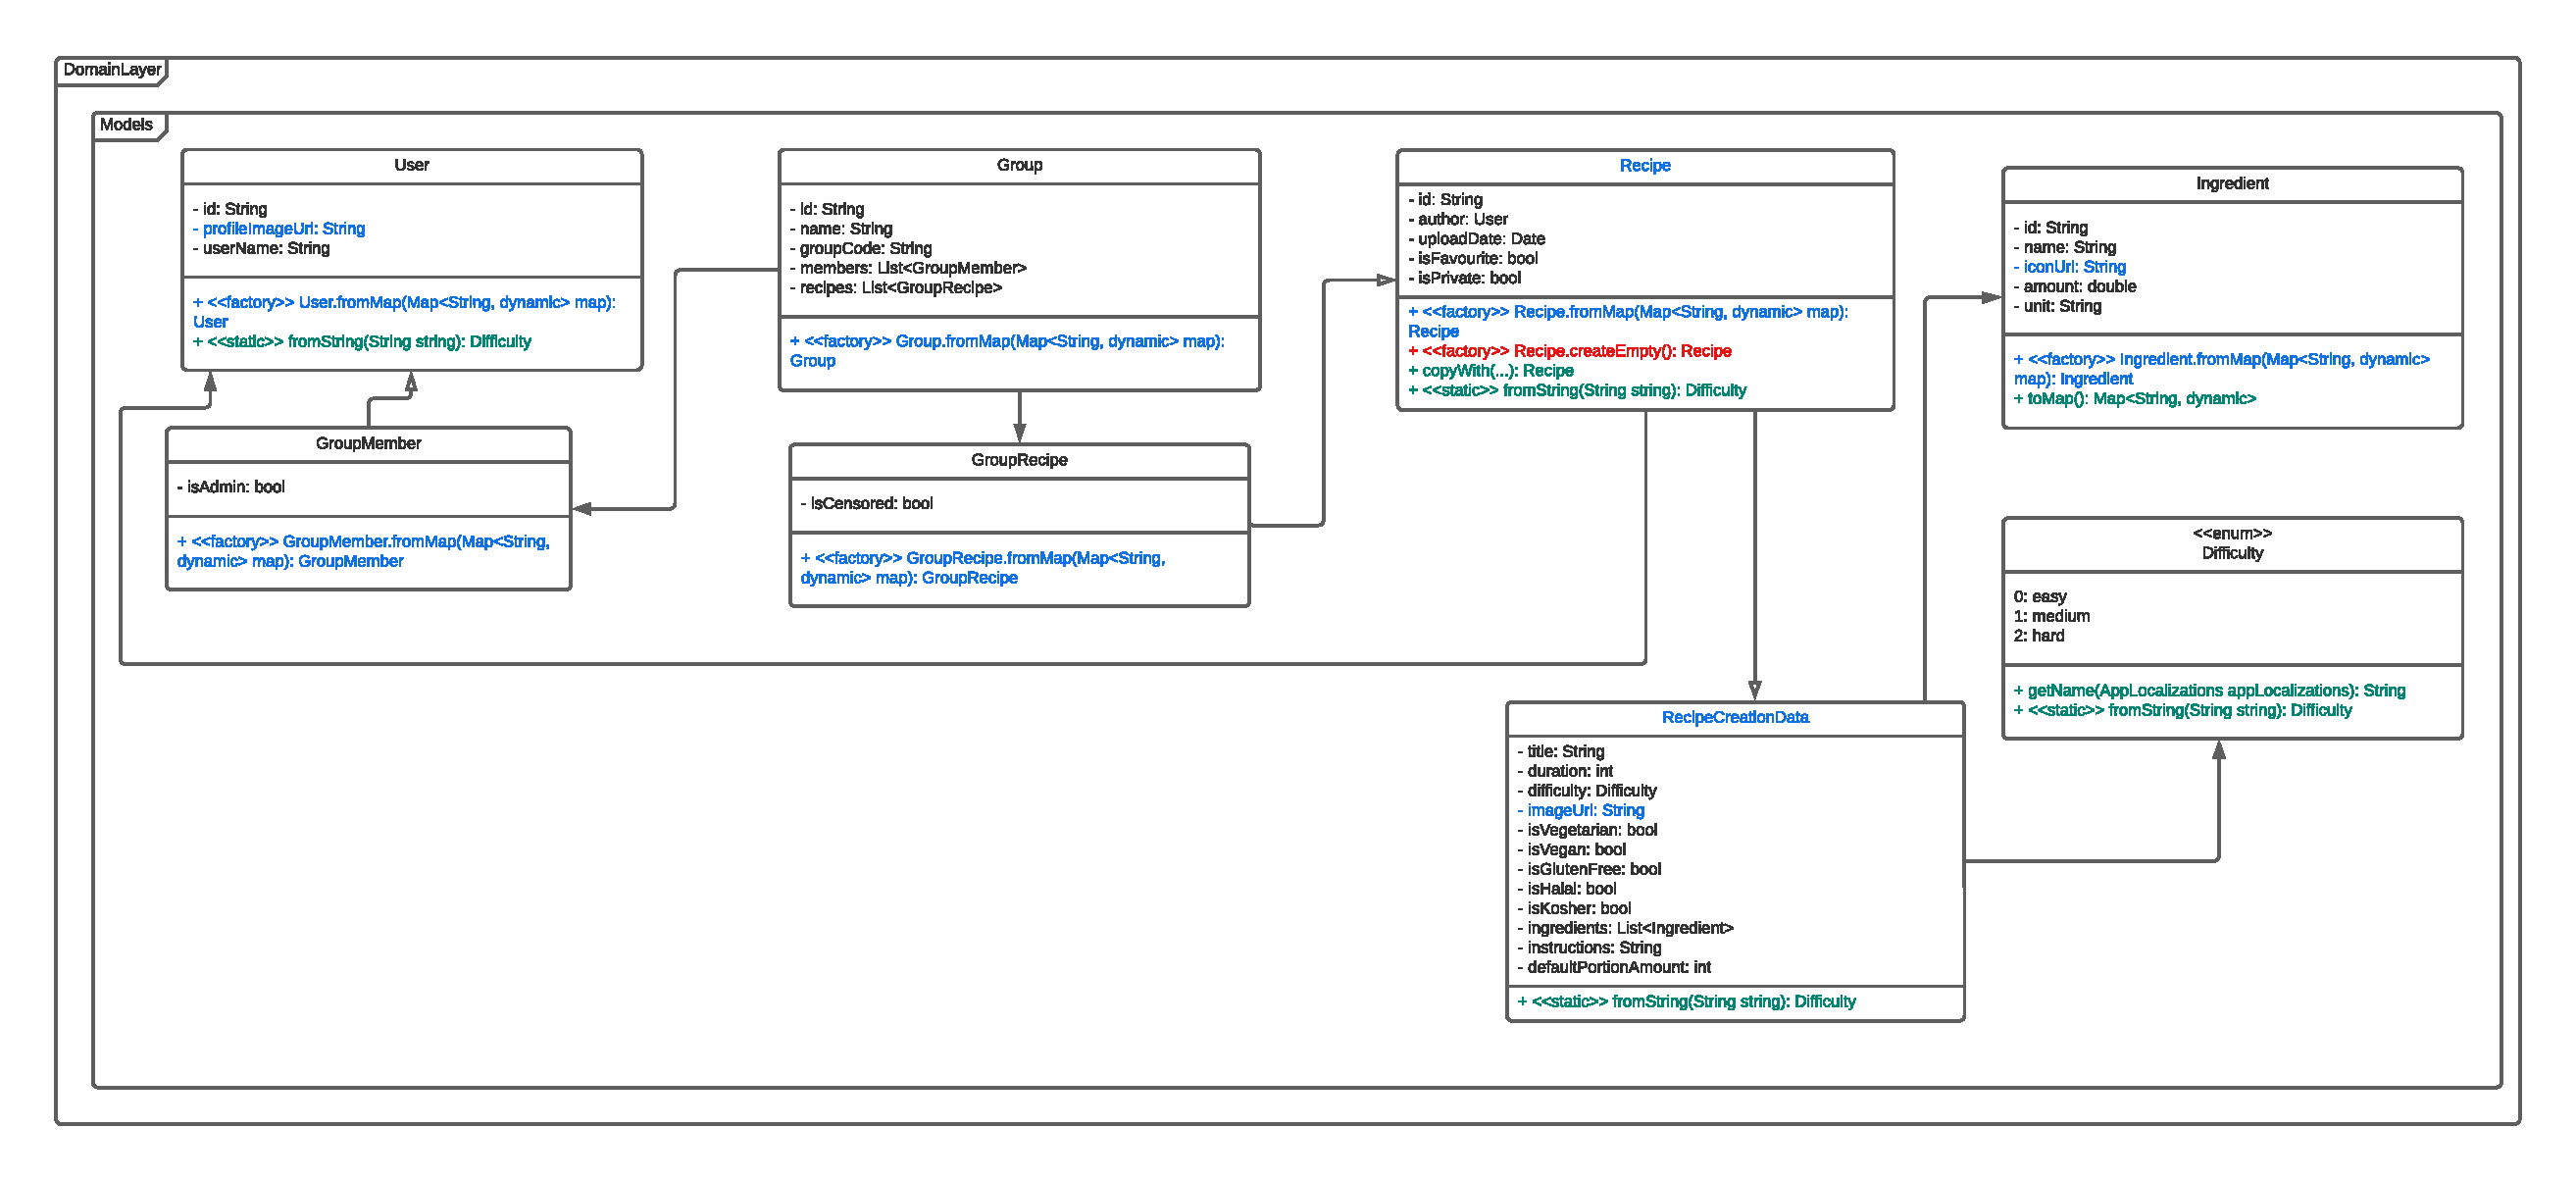
\includegraphics[width=\textwidth]{images/uml/modelLayer.pdf}
    \caption{Änderungen am Modellayer}
    \label{fig:modellayer}
\end{figure}
\paragraph*{\texttt{fromMap(Map<String, dynamic> map)}} Die Factory-Methoden \texttt{fromJson} wurden in \texttt{fromMap} umbenannt, da sie unabhängig von der Serialisierungsmethode sind.
\paragraph*{\texttt{toMap()}} Die statische Methode \texttt{toMap} wurde bei einigen Klassen hinzugefügt, um die Serialisierung zu vereinfachen. Sie gibt ein \texttt{Map<String, dynamic>} zurück, das die Attribute der Klasse enthält.
\paragraph{\texttt{Recipe} und \texttt{RecipeCreationData}}
Die Klasse \texttt{Recipe} wurde in die beiden Klassen \texttt{Recipe} und \texttt{RecipeCreationData} aufgeteilt. Die Klasse \texttt{Recipe} enthält nur noch die Attribute, die ein Rezept nach der Erstellung haben kann, wie zum Beispiel den Author und die Id. Die Klasse erbt von \texttt{RecipeCreationData}, die die Attribute enthält, die ein Rezept bei der Erstellung haben muss, wie Namen oder Anweisungen.
\paragraph{\texttt{Recipe.copyWith(...)}} Die Methode \texttt{copyWith} wurde hinzugefügt, um ein Rezept zu kopieren und dabei einzelne Attribute zu ändern. Die zuändernden Attribute werden als benannte Parameter übergeben.
\paragraph{\texttt{Recipe.createEmpty()}} Die Methode wurde entfernt, da sie nicht mehr benötigt wird.
\paragraph{\texttt{Difficulty.getName(AppLocalizations appLocalizations): String}}
Es handelt sich um eine Methode zum Zurückgeben des Namens der Schwierigkeit in der aktuellen Sprache. Die Sprache wird aus den \texttt{AppLocaliza\-tions} gelesen.
\paragraph{\texttt{Difficulty.fromString(String string)}}
Die statische Methode gibt die Schwierigkeit zurück, die den übergebenen String als Namen hat.
\paragraph{\texttt{User.profileImageUrl}, \texttt{RecipeCreationData.imageUrl} und \texttt{Ingredient.iconUrl}} Wir haben uns dazu entschieden statt den Icons/Bildern nur die URL zu speichern. Damit können wir die Anfragengröße massiv verkleinern. Die Bilder werden erst dann geladen, wenn sie benötigt werden. Ein leerer String bedeutet immer, dass kein Bild gesetzt ist.
\newpage
\subsection{Änderungen am Datalayer}
\begin{figure}[htp]
    \centering
    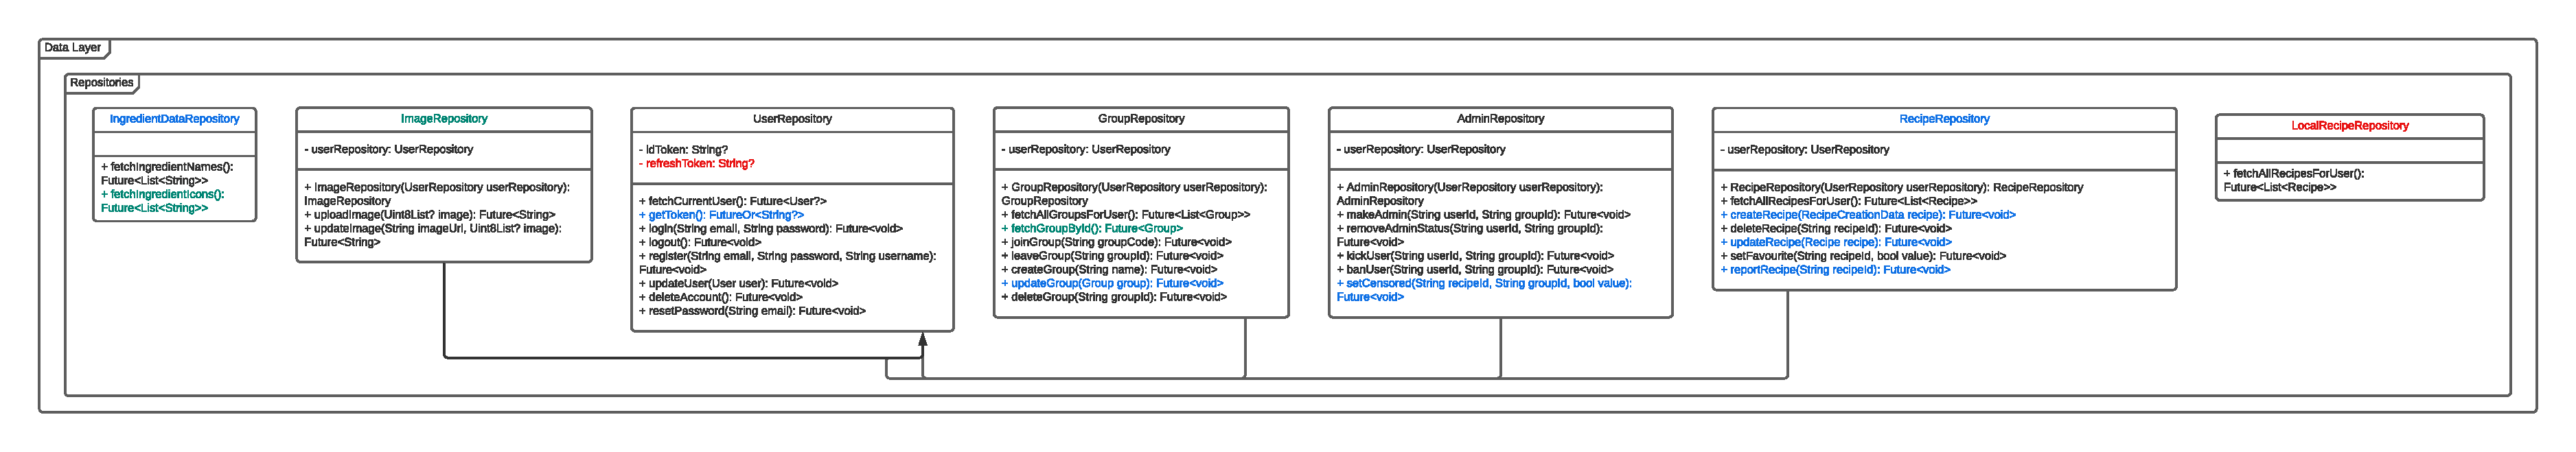
\includegraphics[width=\textwidth]{images/uml/dataLayer.pdf}
    \caption{Änderungen am Datalayer}
    \label{fig:dataLayer}
\end{figure}
\subsubsection{\texttt{RecipeRepository}}
Das Konzept, ein lokales und ein entferntes Repository zu haben, wurde verworfen. Stattdessen gibt es nur noch ein Repository, das auf die Daten des Servers zugreift.
\paragraph{\texttt{createRecipe(RecipeCreationData recipe)}} Die Methode nimmt statt einem \texttt{Recipe} ein Objekt der neuen Klasse \texttt{RecipeCreationData} entgegen, das wirklich nur die benötigten Daten enthält.
\paragraph{\texttt{updateRecipe(Recipe recipe)}} Die Methode nimmt keine Id mehr als Parameter entgegen. Stattdessen wird die Id aus dem übergebenen \texttt{Recipe} gelesen.
\paragraph{\texttt{reportRecipe(String recipeId)}} Die Methode nimmt nur noch die Id des zu meldenden Rezepts entgegen und nicht mehr das gesamte Rezept.
\subsubsection{\texttt{AdminRepository}}
\paragraph{\texttt{setCensored(String recipeId, String groupId, bool value)}} Im Entwurf wurde vergessen, die Id der Gruppe als Parameter hinzuzufügen. Das wurde nun nachgeholt.
\subsubsection{\texttt{GroupRepository}}
\paragraph*{\texttt{fetchGroupById()}} Die Methode wurde hinzugefügt, um eine Gruppe anhand ihrer Id zu laden. Dies ist vor allem für die Gurppen-Detail-Seite nötig.
\paragraph*{\texttt{updateGroup(Group group)}} Die Methode nimmt keine Id mehr als Parameter entgegen. Stattdessen wird die Id aus der übergebenen \texttt{Group} gelesen.
\subsubsection{\texttt{UserRepository}}
\paragraph{\texttt{refreshToken}}
Das Attribut wurde entfernt. Stattdessen wird das Token im Systemspeicher abgelegt, da es nur selten benötigt wird, aber über mehrere Sitzungen hinweg gültig ist.
\paragraph{\texttt{getToken(): FutureOr<String?>}} Die Methode gibt ein \texttt{FutureOr<String?>} zurück, da das Token asynchron geladen werden kann, jedoch nicht muss.
\subsubsection{\texttt{IngredientDataRepository}}
Die Klasse wurde umbenannt, da sie nun nicht mehr nur die Namensvorschläge für Zutaten enthält, sondern auch die für Icon-Urls.
\paragraph{\texttt{fetchIngredientIcons()}} Die Methode wurde hinzugefügt, um die Liste der möglichen Iconpfade zu laden.
\subsubsection{\texttt{ImageRepository}}
Die Klasse wurde hinzugefügt, um es zu ermöglichen, Bilder getrennt vom Rest der Daten hochzuladen oder abzuändern. Die Klasse wird, wie die anderen Repositories, über einen Provider verfügbar gemacht.
\paragraph{\texttt{uploadImage(Uint8List? image)}} Die Methode lädt ein Bild hoch und gibt die URL zurück, unter der es erreichbar ist. Ist das Bild \texttt{null}, ein leerer String zurückgegeben, um diesen im Anschluss für andere Methodenaufrufe zu verwenden.
\paragraph{\texttt{updateImage(String imageUrl, Uint8List? image)}} Die Methode ändert das Bild unter der übergebenen URL ab und gibt den Pfad zurück, unter dem es erreichbar ist. Ist das Bild \texttt{null}, wird ein leerer String zurückgegeben, um diesen im Anschluss für andere Methodenaufrufe zu verwenden.
\newpage
\subsection{Änderungen am Domainlayer}
\begin{figure}[htp]
    \centering
    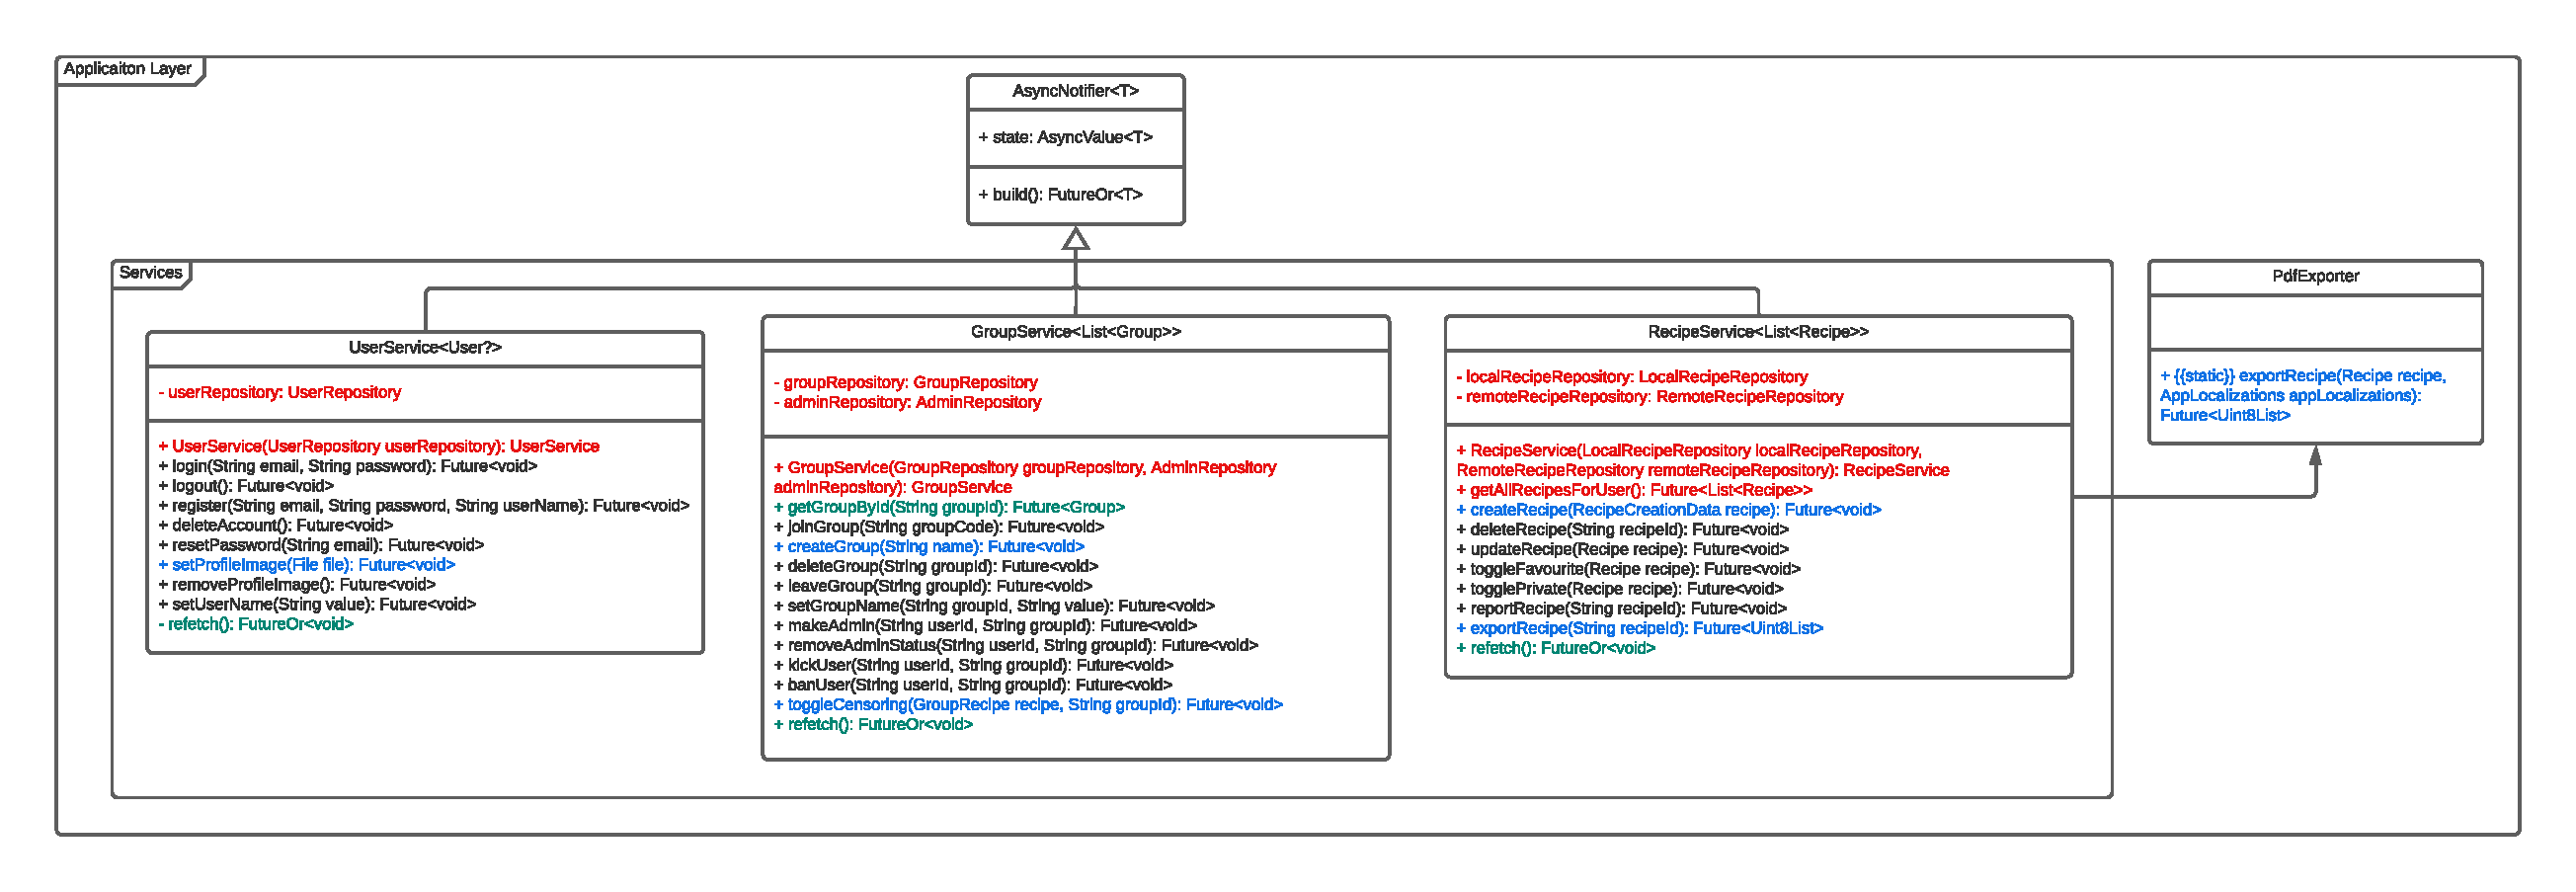
\includegraphics[width=\textwidth]{images/uml/domainLayer.pdf}
    \caption{Änderungen am Domainlayer}
    \label{fig:domainLayer}
\end{figure}
\paragraph{Repository-Objekte und Konstruktoren}
Da alle von \texttt{AsyncNotifier} erbenden Klassen Zugriff auf ein \texttt{ref} Objekt haben, benötigen sie keine Referenz auf die einzelnen Repositories mehr. Stattdessen können sie über dieses Objekt auf die Repositories zugreifen. Somit sind auch die Konstruktoren nicht mehr nötig und wurden entfernt.
\paragraph{\texttt{refetch()}}
Alle Services besitzen eine Methode \texttt{refetch()}, die die gehaltenen Daten neu lädt. Sie ist öffentlich, damit die Daten auch von außen neu geladen werden können. Die einzige Ausnahme bildet dabei der \texttt{UserService}, da dieser nur sich selbst neu laden können muss.
\subsubsection{\texttt{UserService}}
\paragraph*{\texttt{setProfileImage(File file)}}
Der Name des Parameters wurde von \texttt{image} zu \texttt{file} geändert, um zu verdeutlichen, dass es sich um eine Datei handelt. Ansonsten wurde die Methode nicht geändert.
\subsubsection{\texttt{GroupService}}
\paragraph*{\texttt{getGroupById(String groupId)}}
Die Methode wurde hinzugefügt, um eine Gruppe anhand ihrer Id zu laden. Dies ist vor allem für die Gurppen-Detail-Seite nötig.
\paragraph{\texttt{createGroup(String name)}}
Der Parameter wurde von \texttt{title} zu \texttt{name} geändert, um Konsistenz zum Repository zu haben.
\paragraph{\texttt{toggleCensoring(GroupRecipe recipe, String groupId)}}
Der Typ des \texttt{recipe} Parameters wurde von \texttt{Recipe} zu \texttt{GroupRecipe} geändert. Dies ist nötig um Zugriff auf das \texttt{isCensored} Attribut zu haben und entsprechend die richtige Anfrage zu stellen.
\subsubsection{\texttt{RecipeService}}
\paragraph{\texttt{getAllRecipesForUser()}}
Die Methode war fälschlicherweise noch im Entwurf vorhanden. Sie wurde aber durch die \texttt{build()} Methode ersetzt.
\paragraph{\texttt{createRecipe(RecipeCreationData recipe)}}
Es wird die neue Klasse \texttt{RecipeCreationData} verwendet, die nur die benötigten Daten enthält.
\paragraph{\texttt{exportRecipe(String recipeId)}}
Die Klasse gibt nun ein \texttt{Future<Uint8List>} zurück, das die Daten des PDFs enthält. Dies ermöglicht es die Daten anschließend in einer Preview anzuzeigen.
\subsubsection{\texttt{PDFExporter}}
\paragraph{\texttt{exportRecipe(Recipe recipe, AppLocalizations appLocalizations)}}
Es wird nun auch ein \texttt{AppLocalizations} Objekt entgegengenommen, um die Übersetzungen zu laden. Zudem gibt sie auch ein \texttt{Future<Uint8List>} zurück, das die Daten des PDFs enthält. Dies ermöglicht es die Daten anschließend in einer Preview anzuzeigen.
\newpage
\subsection{Änderungen am Presentationlayer}
\begin{figure}[htp]
    \centering
    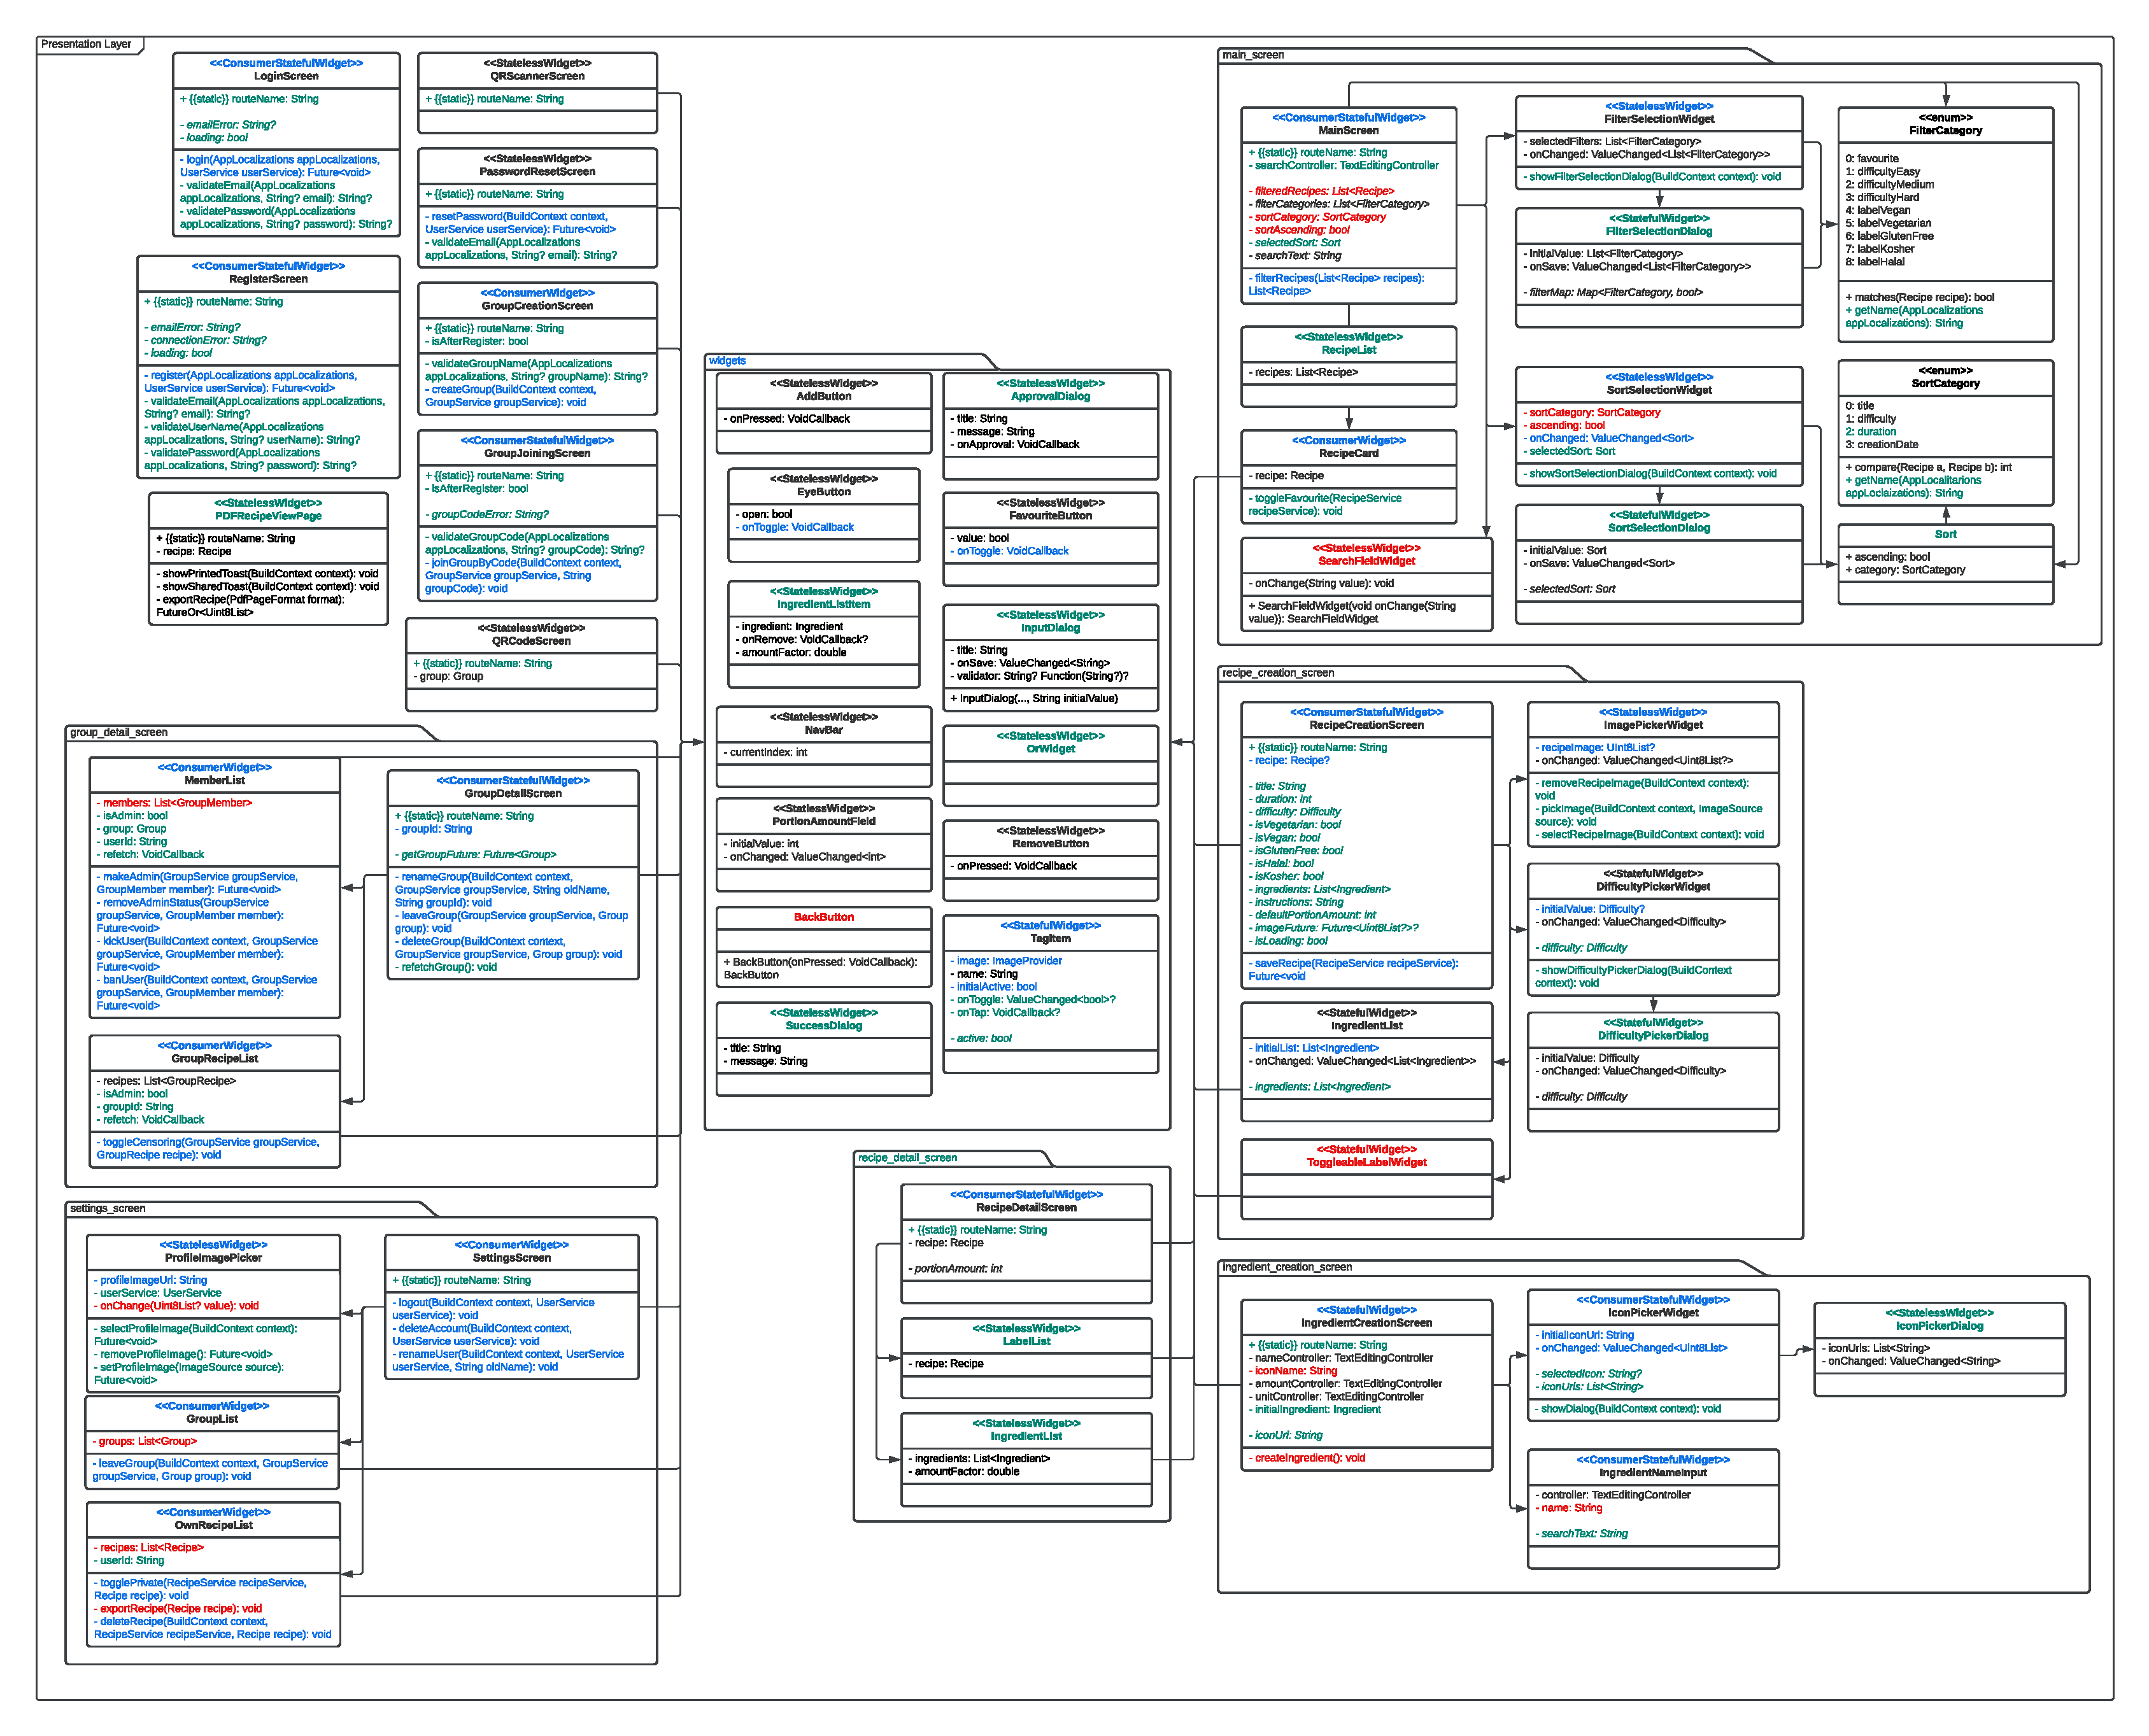
\includegraphics[width=\textwidth]{images/uml/presentationLayer.pdf}
    \caption{Änderungen am Presentationlayer}
    \label{fig:presentationLayer}
\end{figure}
Alle Attribute der Klassen werden in einem Konstruktor gesetzt, der der Übersichtlichkeit halber nicht dargestellt wird. Die Ausnahme bilden die Attribute, die als Zustand der \texttt{StatefulWidgets} oder \texttt{ConsumerStatefulWidgets} gehalten werden. Sie sind daran zu erkennen, dass sie \textit{kursiv} geschrieben sind.
\paragraph{Vererbungen}
Google selbst empfiehlt für Flutter-Widgets keine Vererbung von anderen Widgets zu verwenden. Stattdessen soll die \texttt{build}-Methode des Widgets alle nötigen Anpassungen vornehmen. Dieses Prinzip nennt sich "Composition over Inheritence". Daher wurden die Vererbungen zu Klassen wie \texttt{IconButton} entfernt.
\paragraph{\texttt{ConsumerWidget} und \texttt{ConsumerStatefulWidget}} Die beiden Klassen aus dem \texttt{Riverpod}-Paket wurden an sinnvollen Stellen verwendet, um die Daten aus den Providern laden zu können. \texttt{ConsumerWidget} wird für \texttt{StatelessWidgets} und \texttt{ConsumerStatefulWidget} für \texttt{StatefulWid\-gets} verwendet.
\paragraph{\texttt{routeName}}
Das Attribut wurde jedem Screen hinzugefügt, um die Navigation zu vereinfachen. Es ist öffentlich, damit andere Screens auf den Namen zugreifen können und dem Navigator mitteilen können, welcher Screen als nächstes angezeigt werden soll.
\subsubsection{\texttt{widgets}}
Das zuvor \texttt{ui\_elements} genannte Paket wurde in \texttt{widgets} umbenannt, da dies eine bessere Bezeichnung ist.
\subsubsection*{\texttt{ApprovalDialog}}
Die Klasse stellt ein Pop-Up-Fenster dar, das nach Bestätigung eine Aktion ausführt. Es wird ein Titel und eine Nachricht übergeben. Der Callback wird ausgeführt, wenn der Nutzer die Aktion bestätigt.
\subsubsection*{\texttt{EyeButton}}
\paragraph{\texttt{onToggle}}
Der Callback heißt nicht mehr \texttt{onPressed}, da dieser Bezeichner genauer ist.
\subsubsection*{\texttt{FavouriteButton}}
\paragraph{\texttt{onToggle}}
Der Callback heißt nicht mehr \texttt{onPressed}, da dieser Bezeichner genauer ist.
\subsubsection*{\texttt{IngredientListItem}}
Die Klasse wurde hinzugefügt, um eine Zutat in einer Liste anzuzeigen. Es wird ein \texttt{Ingredient} Objekt übergeben, das die anzuzeigenden Daten enthält. Zudem wird ein Callback übergeben, der ausgeführt wird, wenn der Nutzer auf ein X-Symbol klickt. Ist der Callback \texttt{null}, wird kein X-Symbol angezeigt. Das Attribut \texttt{amountFactor} wird benötigt, um die Zutatenmenge zu skalieren.
\subsubsection*{\texttt{InputDialog}}
Das Widget wird verwendet, um ein Pop-Up-Fenster anzuzeigen, in dem der Nutzer einen Text eingeben kann. Es wird ein Titel übergeben. Der Callback wird ausgeführt, wenn der Nutzer den Text bestätigt. Es kann zudem eine Funktion übergeben werden, die prüft, ob der eingegebene Text gültig ist. Ist dies nicht der Fall, wird der zurückgegebene String als Fehlermeldung angezeigt.
Im Konstruktor kann außerdem ein initialer Text übergeben werden.
\subsubsection*{\texttt{OrWidget}}
Das Widget wurde hinzugefügt, um die häufig verwendete Trennlinie, in deren Mitte "oder" steht zu vereinfachen.
\subsubsection*{\texttt{TagItem}}
Das Tag Item ist nun ein StatefulWidget, da es die Möglichkeit bieten soll, die Farbe des Tags zu ändern, wenn es aktiviert wurde.
\paragraph*{\texttt{imageData}}
Dasehemalige Attribut \texttt{icon} wurde so abgeändert, dass es nun einen \texttt{imageProvider} entgegennimmt, der der ein Bild enthält, das als Icon angezeigt wird.
\paragraph*{\texttt{initialActive}}
Das Attribut \texttt{isActive} wurde umbenannt, da es nun nur noch den initialen Zustand des Tags enthält.
\paragraph*{\texttt{onToggle}}
Der Callback wird ausgeführt, wenn der Nutzer auf das Tag klickt. Er gibt den neuen Zustand des Tags zurück. Ist der Callback \texttt{null}, kann der Zustand des Tags nicht geändert werden.
\paragraph*{\texttt{onTap}}
Der Callback wird ausgeführt, wenn der Nutzer auf das Tag klickt. Ist der Callback \texttt{null}, kann keine eigene Aktion beim Antippen ausgeführt werden.
\paragraph*{\texttt{active}}
Der Zustand des Widgets. Ist er wahr, so wird das Widget mit grünem Hintergrund angezeigt. Ist er falsch, wird es mit grauem Hintergrund angezeigt.
\subsubsection*{\texttt{BackButton}}
Das Widget wurde entfernt, da Flutter bereits ein \texttt{BackButton} Widget bereitstellt.
\subsubsection*{\texttt{SuccessDialog}}
Das Widget dient dazu, eine Erfolgsmeldung anzuzeigen. Es wird ein Titel und eine Nachricht übergeben.
\subsubsection{\texttt{LoginScreen}}
Das Widget ist nun ein \texttt{ConsumerStatefulWidget}, da es nun Fehlermeldung und Ladezustand verwaltet und auf die Methoden des \texttt{UserService} zugreift.
\paragraph{\texttt{emailError}}
Das Attribut wurde hinzugefügt, um die Fehlermeldung für die E-Mail-Adresse zu speichern und dynamisch anzuzeigen.
\paragraph{\texttt{loading}}
Das Attribut wurde hinzugefügt, um den Ladezustand zu speichern und dynamisch anzuzeigen.
\paragraph{\texttt{login(AppLocalizations appLocalizations, UserService userService)}}
Es wird nun ein \texttt{AppLocalizations} Objekt übergeben, um die Übersetzungen zu laden. Zudem wird ein \texttt{UserSer\-vice} Objekt entgegengenommen, um auf die Methoden des Services zugreifen zu können. Dieses wurde zuvor aus dem Provider geladen.
\paragraph{\texttt{validateEmail(AppLocalizations appLocalizations, String? email)}}
Die Methode dient dazu, eine E-Mail-Adresse zu validieren und gibt eine Fehlermeldung zurück, wenn die E-Mail-Adresse ungültig ist. Sie nimmt ein \texttt{AppLocalizations} Objekt entgegen, um die Übersetzungen zu laden, sowie die E-Mail-Adresse, die validiert werden soll.
\paragraph{\texttt{validatePassword(AppLocalizations appLocalizations, String? password)}}
Die Methode dient dazu, ein Passwort zu validieren und gibt eine Fehlermeldung zurück, wenn das Passwort ungültig ist. Sie nimmt ein \texttt{AppLocalizations} Objekt entgegen, um die Übersetzungen zu laden, sowie das Passwort, das validiert werden soll.
\subsubsection{\texttt{RegisterScreen}}
Die Klasse ist nun ein \texttt{ConsumerStatefulWidget}, da sie Fehlermeldungen und Ladezustand verwaltet und auf die Methoden des \texttt{UserService} zugreift.
\paragraph{\texttt{emailError}}
Das Attribut wurde hinzugefügt, um die Fehlermeldung für die E-Mail-Adresse zu speichern und dynamisch anzuzeigen.
\paragraph{\texttt{connectionError}}
Das Attribut wurde hinzugefügt, um die Fehlermeldung für die Verbindungsprobleme zu speichern und dynamisch anzuzeigen.
\paragraph{\texttt{loading}}
Das Attribut wurde hinzugefügt, um den Ladezustand zu speichern und dynamisch anzuzeigen.
\paragraph{\texttt{register(AppLocalizations appLocalizations, UserService userService)}}
Es wird nun ein \texttt{AppLocalizations} Objekt übergeben, um die Übersetzungen zu laden. Zudem wird ein \texttt{UserSer\-vice} Objekt entgegengenommen, um auf die Methoden des Services zugreifen zu können. Dieses wurde zuvor aus dem Provider geladen.
\paragraph{\texttt{validateEmail(AppLocalizations appLocalizations, String? email)}}
Die Methode dient dazu, eine E-Mail-Adresse zu validieren und gibt eine Fehlermeldung zurück, wenn die E-Mail-Adresse ungültig ist. Sie nimmt ein \texttt{AppLocalizations} Objekt entgegen, um die Übersetzungen zu laden, sowie die E-Mail-Adresse, die validiert werden soll.
\paragraph*{\texttt{validateUserName(AppLocalizations appLocalizations, String? userName)}}
Die Methode dient dazu, einen Benutzernamen zu validieren und gibt eine Fehlermeldung zurück, wenn der Benutzername ungültig ist. Sie nimmt ein \texttt{AppLocalizations} Objekt entgegen, um die Übersetzungen zu laden, sowie den Benutzernamen, der validiert werden soll.
\paragraph{\texttt{validatePassword(AppLocalizations appLocalizations, String? password)}}
Die Methode dient dazu, ein Passwort zu validieren und gibt eine Fehlermeldung zurück, wenn das Passwort ungültig ist. Sie nimmt ein \texttt{AppLocalizations} Objekt entgegen, um die Übersetzungen zu laden, sowie das Passwort, das validiert werden soll.
\subsubsection{\texttt{PasswordResetScreen}}
\paragraph*{\texttt{resetPassword(AppLocalizations appLocalizations, UserService userService)}}
Es wird nun ein \texttt{AppLocalizations} Objekt übergeben, um die Übersetzungen zu laden. Zudem wird ein \texttt{UserSer\-vice} Objekt entgegengenommen, um auf die Methoden des Services zugreifen zu können. Dieses wurde zuvor aus dem Provider geladen.
\paragraph{\texttt{validateEmail(AppLocalizations appLocalizations, String? email)}}
Die Methode dient dazu, eine E-Mail-Adresse zu validieren und gibt eine Fehlermeldung zurück, wenn die E-Mail-Adresse ungültig ist. Sie nimmt ein \texttt{AppLocalizations} Objekt entgegen, um die Übersetzungen zu laden, sowie die E-Mail-Adresse, die validiert werden soll.
\subsubsection{\texttt{GroupCreationScreen}}
Die Klasse ist nun ein ConsumerWidget, da sie auf die Methoden des \texttt{GroupService} zugreift.
\paragraph*{\texttt{isAfterRegister}}
Das Attribut wurde hinzugefügt, um zu speichern, ob die Seite nach der Registrierung angezeigt wird. Davon hängt ab, ob ein Überspringen-Button angezeigt wird und wohin nach Abschluss der Gruppenerstellung navigiert wird.
\paragraph*{\texttt{validateGroupName(AppLocalizations appLocalizations, String? groupName)}}
Die Methode dient dazu, einen Gruppennamen zu validieren und gibt eine Fehlermeldung zurück, wenn der Gruppenname ungültig ist. Sie nimmt ein \texttt{AppLocalizations} Objekt entgegen, um die Übersetzungen zu laden, sowie den Gruppennamen, der validiert werden soll.
\paragraph{\texttt{createGroup(AppLocalizations appLocalizations, GroupService groupService)}}
Es wird nun ein \texttt{AppLocalizations} Objekt übergeben, um die Übersetzungen zu laden. Zudem wird ein \texttt{GroupService} Objekt entgegengenommen, um auf die Methoden des Services zugreifen zu können. Dieses wurde zuvor aus dem Provider geladen.
\subsubsection{\texttt{GroupJoiningScreen}}
Die Klasse ist nun ein ConsumerStatefulWidget, da sie auf die Methoden des \texttt{GroupService} zugreift und eine Fehlermeldung dynamisch verwaltet und anzeigt.
\paragraph{\texttt{isAfterRegister}}
Das Attribut wurde hinzugefügt, um zu speichern, ob die Seite nach der Registrierung angezeigt wird. Davon hängt ab, ob ein Überspringen-Button angezeigt wird und wohin nach Abschluss der Gruppenerstellung navigiert wird.
\paragraph{\texttt{groupCodeError}}
Das Attribut wurde hinzugefügt, um die Fehlermeldung für den Gruppencode zu speichern und dynamisch anzuzeigen.
\paragraph*{\texttt{validateGroupCode(AppLocalizations appLocalizations, String? groupCode)}}
Die Methode dient dazu, einen Gruppencode zu validieren und gibt eine Fehlermeldung zurück, wenn der Gruppencode ungültig ist. Sie nimmt ein \texttt{AppLocalizations} Objekt entgegen, um die Übersetzungen zu laden, sowie den Gruppencode, der validiert werden soll.
\paragraph{\texttt{joinGroup(AppLocalizations appLocalizations, GroupService groupService,\\ String      groupCode)}}
Es wird nun ein \texttt{AppLocalizations} Objekt übergeben, um die Übersetzungen zu laden. Zudem wird ein \texttt{GroupService} Objekt entgegengenommen, um auf die Methoden des Services zugreifen zu können. Dieses wurde zuvor aus dem Provider geladen.
\subsubsection{\texttt{PDFRecipeViewPage}}
Die Klasse wurde hinzugefügt, um ein Rezept als PDF anzuzeigen und verschiedene Optionen zum Drucken, etc. zur Verfügung zu stellen. Es wird ein Rezept übergeben, das angezeigt werden soll.
\subsubsection{\texttt{group\_detail\_screen}}
\subsubsection*{\texttt{GroupDetailScreen}}
Die Klasse ist nun ein ConsumerStatefulWidget, da sie auf die Methoden des \texttt{GroupService} zugreift und einen Zustand enthält, von dem abhängt, was angezeigt wird.
\paragraph{\texttt{groupId}}
Es wird nur noch die Id der Gruppe übergeben statt der gesamten Gruppe. Die Gruppe wird nun im Widget selbst geladen. Dadurch kann die Gruppe auch neu geladen werden, wenn sich die Daten ändern.
\paragraph{\texttt{getGroupFuture}}
Das Attribut wurde hinzugefügt, um die Gruppe zu laden. Wird es neu gesetzt, wird die Gruppe neu geladen. Es fungiert als Zustand des Widgets.
\paragraph{\texttt{renameGroup(BuildContext context, GroupService groupService, String oldName,\\ String groupId)}}
Die Methode nimmt nun den \texttt{BuildContext} entgegen, um die Übersetzungen zu laden und ein Pop-Up-Fenster zu öffnen, in dem der neue Name eingegebe wird. Den Initialwert dieses Dialogs bildet der alte Name. Zudem wird ein \texttt{GroupService} Objekt entgegengenommen, um auf die Methoden des Services zugreifen zu können. Dieses wurde zuvor aus dem Provider geladen. Die Id der Gruppe wird ebenfalls übergeben.
\paragraph{\texttt{leaveGroup(BuildContext context, GroupService groupService, String groupId)}}
Die Methode nimmt nun den \texttt{BuildContext} entgegen, um die Übersetzungen zu laden und ein Pop-Up-Fenster zu öffnen, in dem der Nutzer bestätigen muss, dass er die Gruppe verlassen möchte. Zudem wird ein \texttt{GroupService} Objekt entgegengenommen, um auf die Methoden des Services zugreifen zu können. Dieses wurde zuvor aus dem Provider geladen. Die Id der Gruppe wird ebenfalls übergeben.
\paragraph{\texttt{deleteGroup(BuildContext context, GroupService groupService, Group group)}}
Die Methode nimmt nun den \texttt{BuildContext} entgegen, um die Übersetzungen zu laden und ein Pop-Up-Fenster zu öffnen, in dem der Nutzer bestätigen muss, dass er die Gruppe löschen möchte. Zudem wird ein \texttt{GroupService} Objekt entgegengenommen, um auf die Methoden des Services zugreifen zu können. Dieses wurde zuvor aus dem Provider geladen. Die Gruppe wird ebenfalls übergeben.
\paragraph{\texttt{refetchGroup()}}
Die Methode lädt die Gruppe neu. Dies wird nach jeder Änderung der Gruppe ausgeführt.
\subsubsection*{\texttt{GroupRecipeList}}
Die Klasse ist nun ein ConsumerWidget, da sie auf die Methoden des \texttt{GroupService} zugreift.
\paragraph{\texttt{isAdmin}}
Die Klasse hat nun ein Attribut, das bestimmt, ob die Administratoraktionen angezeigt werden sollen.
\paragraph{\texttt{groupId}}
Es wird die Id der Gruppe gespeichert, um später Methoden mit dieser Id auszuführen.
\paragraph{\texttt{refetch}}
Der Callback der nach dem Durchführen einer Aktion ausgeführt wird, um die Daten neu zu laden.
\paragraph{\texttt{toggleCensoring(GroupService groupService, GroupRecipe recipe)}}
Die Methode nimmt nun ein \texttt{GroupService} Objekt entgegen, um auf die Methoden des Services zugreifen zu können. Dieses wurde zuvor aus dem Provider geladen. Zudem wird ein \texttt{GroupRecipe} Objekt übergeben, das die Daten des Rezepts enthält, dessen Sichtbarkeit geändert werden soll.
\subsubsection*{\texttt{MemberList}}
Die Klasse ist nun ein ConsumerWidget, da sie auf die Methoden des \texttt{GroupService} zugreift.
\paragraph{\texttt{members}}
Das Attribut wurde entfernt, da das Widget die Mitglieder aus dem \texttt{group}-Objekt lädt.
\paragraph{\texttt{isAdmin}}
Die Klasse hat nun ein Attribut, das bestimmt, ob die Administratoraktionen angezeigt werden sollen.
\paragraph{\texttt{group}}
Es wird die Gruppe gespeichert, um später Methoden mit dieser Gruppe auszuführen und die Mitglieder zu laden.
\paragraph{\texttt{userId}}
Die Id des Nutzers wird gespeichert, um den aktuellen Nutzer in der Liste speziell hervorzuheben.
\paragraph{\texttt{refetch}}
Der Callback der nach dem Durchführen einer Aktion ausgeführt wird, um die Daten neu zu laden.
\paragraph{\texttt{makeAdmin(GroupService groupService, GroupMember member)}}
Die Methode nimmt nun ein \texttt{GroupService} Objekt entgegen, um auf die Methoden des Services zugreifen zu können. Dieses wurde zuvor aus dem Provider geladen. Zudem wird ein \texttt{GroupMember} Objekt übergeben, das die Daten des Mitglieds enthält, das zum Administrator ernannt werden soll.
\paragraph{\texttt{removeAdminStatus(GroupService groupService, GroupMember member)}}
Die Methode bekommt nun ein \texttt{GroupService} Objekt mitgegeben, um auf die Methoden des Services zugreifen zu können. Dieses wurde zuvor aus dem Provider geladen. Zudem wird ein \texttt{GroupMember} Objekt übergeben, das die Daten des Mitglieds enthält, das der Administratorstatus entzogen werden soll.
\paragraph{\texttt{kickUser(GroupService groupService, GroupMember member)}}
Die Methode nimmt nun ein \texttt{GroupService} Objekt entgegen, um auf die Methoden des Services zugreifen zu können. Dieses wurde zuvor aus dem Provider geladen. Zudem wird ein \texttt{GroupMember} Objekt übergeben, das die Daten des Mitglieds enthält, das gekickt werden soll.
\paragraph{\texttt{banUser(GroupService groupService, GroupMember member)}}
Die Methode nimmt nun ein \texttt{GroupService} Objekt entgegen, um auf die Methoden des Services zugreifen zu können. Dieses wurde zuvor aus dem Provider geladen. Zudem wird ein \texttt{GroupMember} Objekt übergeben, das die Daten des Mitglieds enthält, das gebannt werden soll.
\subsubsection{\texttt{settings\_screen}}
\subsubsection*{\texttt{SettingsScreen}}
Die Klasse ist nun ein ConsumerWidget, da sie auf die Methoden des \texttt{UserService} zugreift.
\paragraph{\texttt{logout(BuildContext context, UserService userService)}}
Die Methode nimmt nun ein \texttt{UserService} Objekt entgegen, um auf die Methoden des Services zugreifen zu können. Dieses wurde zuvor aus dem Provider geladen. Zudem wird der \texttt{BuildContext} übergeben, um die Übersetzungen zu laden, ein Pop-Up-Fenster anzuzeigen und die Navigation zu ermöglichen.
\paragraph{\texttt{deleteAccount(BuildContext context, UserService userService)}}
Die Methode nimmt nun ein \texttt{UserService} Objekt entgegen, um auf die Methoden des Services zugreifen zu können. Dieses wurde zuvor aus dem Provider geladen. Zudem wird der \texttt{BuildContext} übergeben, um die Übersetzungen zu laden, ein Pop-Up-Fenster anzuzeigen und die Navigation zu ermöglichen.
\paragraph{\texttt{renameUser(BuildContext context, UserService userService, String oldName)}}
Die Methode nimmt nun ein \texttt{UserService} Objekt entgegen, um auf die Methoden des Services zugreifen zu können. Dieses wurde zuvor aus dem Provider geladen. Zudem wird der \texttt{BuildContext} übergeben, um die Übersetzungen zu laden und ein Pop-Up-Fenster anzuzeigen. Der alte Name wird ebenfalls übergeben, um den Initialwert der Texteingabe zu setzen.
\subsubsection*{\texttt{ProfileImagePicker}}
Die Klasse ist nun ein StatelessWidget, da sie keinen Zustand mehr verwaltet.
\paragraph{\texttt{profileImageUrl}}
Das Widget bekommt nur noch die URL übergeben und nicht mehr das gesamte Bild. Außerdem ändert sie diese nicht selbst, sondern bekommt sie vom Parentwidget übergeben.
\paragraph{\texttt{userService}}
Das Widget bekommt nun ein \texttt{UserService} Objekt übergeben, um auf die Methoden des Services zugreifen zu können. Dieses wurde zuvor vom Parentwidget aus dem Provider geladen.
\paragraph{\texttt{onChange(Uint8List? value)}}
Der Callback wird nicht mehr verwendet. Die Zustandsverwaltung erfolgt nun nämlich über das Parentwidget, welches wiederum seinen Zustand aus dem UserService liest.
\paragraph{\texttt{selectProfileImage(BuildContext context)}}
Die Methode wurde hinzugefügt, um ein Pop-Up-Fenster anzuzeigen, in dem der Nutzer verschiedene Auswahlmöglichkeiten hat, um ein Bild auszuwählen oder zu löschen. Zu diesem Zweck wird der \texttt{BuildContext} übergeben, um die Übersetzungen zu laden und das Pop-Up-Fenster anzuzeigen.
\paragraph*{\texttt{removeProfileImage()}}
Die Methode löscht das Profilbild des Nutzers.
\paragraph*{\texttt{setProfileImage(ImageSource source)}}
Die Methode lädt ein Bild hoch und setzt es als Profilbild des Nutzers. Dazu wird die Quelle des Bildes übergeben, die entweder die Kamera oder die Galerie ist.
\subsubsection*{\texttt{GroupList}}
Die Klasse ist nun ein ConsumerWidget, da sie auf die Methoden des \texttt{GroupService} zugreift.
\paragraph{\texttt{groups}}
Das Attribut wurde entfernt, stattdessen wird die Liste der Gruppen aus dem \texttt{GroupSer\-vice} geladen.
\paragraph{\texttt{leaveGroup(BuildContext context, GroupService groupService, Group group)}}
Die Methode nimmt nun den \texttt{BuildContext} entgegen, um die Übersetzungen zu laden und ein Pop-Up-Fenster zu öffnen, in dem der Nutzer bestätigen muss, dass er die Gruppe verlassen möchte. Zudem wird ein \texttt{GroupService} Objekt entgegengenommen, um auf die Methoden des Services zugreifen zu können. Dieses wurde zuvor aus dem Provider geladen. Die Gruppe wird ebenfalls übergeben, um zu wissen, welche Gruppe verlassen werden soll.
\subsubsection*{\texttt{OwnRecipeList}}
Die Klasse ist nun ein ConsumerWidget, da sie keinen eigenen Zustand mehr verwaltet, aber auf die Methoden des \texttt{RecipeService} zugreift.
\paragraph{\texttt{recipes}}
Das Attribut wurde entfernt, stattdessen wird die Liste der Rezepte aus dem \texttt{RecipeSer\-vice} geladen.
\paragraph{\texttt{userId}}
Die Id des Nutzers wird gespeichert, um die Rezeptliste nach denen des Nutzers zu filtern.
\paragraph{\texttt{togglePrivate(RecipeService recipeService, Recipe recipe)}}
Die Methode nimmt nun ein \texttt{RecipeService} Objekt entgegen, um auf die Methoden des Services zugreifen zu können. Dieses wurde zuvor aus dem Provider geladen. Das Rezept wird ebenfalls übergeben, um zu wissen, welches Rezept ausgeblendet werden soll.
\paragraph{\texttt{exportRecipe(Recipe recipe)}}
Die Methode wurde gelöscht, da diese Logik nun im \texttt{PDFRecipe\-ViewPage} enthalten ist.
\paragraph{\texttt{deleteRecipe(BuildContext context, RecipeService recipeService, Recipe recipe)}\\}
Die Methode nimmt nun den \texttt{BuildContext} entgegen, um die Übersetzungen zu laden und ein Pop-Up-Fenster zu öffnen, in dem der Nutzer bestätigen muss, dass er das Rezept löschen möchte. Zudem wird ein \texttt{RecipeService} Objekt entgegengenommen, um auf die Methoden des Services zugreifen zu können. Dieses wurde zuvor aus dem Provider geladen. Das Rezept wird ebenfalls übergeben, um zu wissen, welches Rezept gelöscht werden soll.
\subsubsection{\texttt{recipe\_detail\_screen}}
Es wurde ein weiteres Paket angelegt, das die Widgets für die Rezept-Detail-Ansicht enthält.
\subsubsection*{\texttt{RecipeDetailScreen}}
Das Widget ist nun ein ConsumerStatefulWidget, da es auf die Methoden des \texttt{UserService} zugreift, um zu wissen, ob es sich um ein Rezept des Nutzers handelt und somit bearbeitbar ist.
\subsubsection*{\texttt{LabelList}}
Die Klasse wurde hinzugefügt, um die aktiven Labels des Rezept anzuzeigen. Es wird das Rezept übergeben, dessen Labels angezeigt werden sollen.
\subsubsection*{\texttt{IngredientList}}
Die Klasse wurde hinzugefügt, um die Zutaten des Rezepts anzuzeigen. Es wird die Liste der Zutaten übergeben, die angezeigt werden sollen und der Faktor, mit dem die Zutatenmengen multipliziert werden sollen.
\subsubsection{\texttt{main\_screen}}
\subsubsection*{\texttt{MainScreen}}
Die Klasse ist nun ein ConsumerStatefulWidget, da sie auf die Methoden des \texttt{RecipeService} zugreift.
\paragraph*{\texttt{searchController}}
Der Controller wurde hinzugefügt, um den Suchtext zu verwalten. Er wird zum Beispiel verwendet um die Suche zurückzusetzen.
\paragraph{\texttt{filteredRecipes}}
Das Attribut wurde entfernt, stattdessen wird die Liste der Rezepte aus dem \texttt{RecipeService} geladen und in der \texttt{build}-Methode gefiltert.
\paragraph{\texttt{sortCategory}, \texttt{sortAscending} und \texttt{selectedSort}} Die Kategorie und Richtung der Sortierung wurden in einem \texttt{Sort}-Objekt zusammengefasst.
\paragraph{\texttt{filterRecipes(List<Recipe> recipes)}}
Die Methode wurde umbenannt und nimmt nun eine Liste von Rezepten entgegen, die gefiltert werden soll. Sie gibt die gefilterte Liste zurück.
\subsubsection*{\texttt{RecipeList}}
Die Klasse stellt eine Liste der Rezeptkarten dar. Dazu nimmt sie eine Liste der Rezepte entgegen.
\paragraph{\texttt{RecipeCard}}
Die Klasse ist nun ein ConsumerWidget, da sie auf die Methoden des \texttt{RecipeService} zugreift.
\paragraph{\texttt{toggleFavourite(RecipeService recipeService, Recipe recipe)}}
Die Methode dient dazu den Favoritenstatus des Rezeptes zu ändern. Sie nimmt ein \texttt{RecipeService} Objekt entgegen, um auf die Methoden des Services zugreifen zu können. Dieses wurde zuvor aus dem Provider geladen. Das Rezept wird ebenfalls übergeben, um zu wissen, welches Rezept favorisiert werden soll.
\subsubsection*{\texttt{SearchFieldWidget}}
Das Widget wurde verworfen, und wird jetzt im \texttt{MainScreen} direkt implementiert.
\subsubsection*{\texttt{FilterSelectionWidget}}
Das Widget ist jetzt ein StatelessWidget, da es keinen eigenen Zustand mehr verwaltet, sondern diesen von außen übergeben bekommt.
\paragraph{\texttt{showFilterSelectionDialog(BuildContext context)}}
Die Methode wurde hinzugefügt, um ein Pop-Up-Fenster anzuzeigen, in dem der Nutzer die Filtereinstellungen ändern kann. Zu diesem Zweck wird der \texttt{BuildContext} übergeben.
\subsubsection*{\texttt{FilterSelectionDialog}}
Das Widget wurde hinzugefügt, um ein Pop-Up-Fenster anzuzeigen, in dem der Nutzer die Filtereinstellungen ändern kann. Es wird eine Liste and Filterkategorien übergeben, das die initialen Filtereinstellungen enthält. Zudem wird ein Callback übergeben, das ausgeführt wird, wenn der Nutzer die Filtereinstellungen speichert. Die aktuell ausgewählten Filter werden in einer Map gespeichert, die dann beim Ausführen des Callbacks umgewandelt wird.
\subsubsection*{\texttt{SortSelectionWidget}}
Das Widget ist jetzt ein StatelessWidget, da es keinen eigenen Zustand mehr verwaltet, sondern diesen von außen übergeben bekommt.
\paragraph{\texttt{sortCategory}, \texttt{ascending} und \texttt{selectedSort}} Die Kategorie und Richtung der Sortierung wurden in einem \texttt{Sort}-Objekt zusammengefasst.
\paragraph{\texttt{onChanged}}
Der Callback gibt nun ein \texttt{Sort}-Objekt zurück, das die neuen Sortiereinstellungen enthält.
\paragraph{\texttt{showSortSelectionDialog(BuildContext context)}}
Die Methode wurde hinzugefügt, um ein Pop-Up-Fenster anzuzeigen, in dem der Nutzer die Sortiereinstellungen ändern kann. Zu diesem Zweck wird der \texttt{BuildContext} übergeben.
\subsubsection*{\texttt{SortSelectionDialog}}
Das Widget wurde hinzugefügt, um ein Pop-Up-Fenster anzuzeigen, in dem der Nutzer die Sortiereinstellungen ändern kann. Es wird ein \texttt{Sort}-Objekt übergeben, das die initialen Sortiereinstellungen enthält. Zudem wird ein Callback übergeben, das ausgeführt wird, wenn der Nutzer die Sortiereinstellungen speichert. Die aktuell ausgewählten Sortiereinstellungen werden in einem \texttt{Sort}-Objekt gespeichert, das dann beim Ausführen des Callbacks übergeben wird.
\subsubsection*{\texttt{FilterCategory}}
\paragraph*{\texttt{getName(AppLocalizations appLocalizations)}}
Die Methode wurde hinzugefügt, um den Namen der Kategorie zu laden. Dazu wird ein \texttt{AppLocalizations} Objekt übergeben, um die Übersetzungen zu laden.
\subsubsection*{\texttt{SortCategory}}
\paragraph*{\texttt{duration}}
Es ist nun auch möglich nach der Dauer eines Rezeptes zu sortieren. Dazu wurde das Attribut hinzugefügt.
\paragraph*{\texttt{getName(AppLocalizations appLocalizations)}}
Die Methode wurde hinzugefügt, um den Namen der Kategorie zu laden. Dazu wird ein \texttt{AppLocalizations} Objekt übergeben, um die Übersetzungen zu laden.
\subsubsection*{\texttt{Sort}}
Die Klasse wurde hinzugefügt, um die Sortiereinstellungen zu speichern. Sie enthält die Kategorie und die Richtung der Sortierung.
\subsubsection{\texttt{recipe\_creation\_screen}}
\subsubsection*{\texttt{RecipeCreationScreen}}
Die Klasse ist nun ein ConsumerStatefulWidget, da sie auf die Methoden des \texttt{RecipeService} zugreift und die eingegebenen Werte verwalten muss.
\paragraph{\texttt{recipe}}
Das Attribut dient nun dazu, ein Rezept übergeben zu können, das bearbeitet werden soll. Ist es \texttt{null}, so wird ein neues Rezept erstellt.
\paragraph{\texttt{title}}
Das Attribut wurde hinzugefügt, um den Titel des Rezepts zu speichern.
\paragraph{\texttt{duration}}
Das Attribut wurde hinzugefügt, um die Dauer des Rezepts zu speichern.
\paragraph{\texttt{difficulty}}
Das Attribut wurde hinzugefügt, um die Schwierigkeit des Rezepts zu speichern.
\paragraph{\texttt{isVegetarian}}
Das Attribut wurde hinzugefügt, um zu speichern, ob das Rezept vegetarisch ist.
\paragraph{\texttt{isVegan}}
Das Attribut wurde hinzugefügt, um zu speichern, ob das Rezept vegan ist.
\paragraph{\texttt{isGlutenFree}}
Das Attribut wurde hinzugefügt, um zu speichern, ob das Rezept glutenfrei ist.
\paragraph{\texttt{isHalal}}
Das Attribut wurde hinzugefügt, um zu speichern, ob das Rezept halal ist.
\paragraph{\texttt{isKosher}}
Das Attribut wurde hinzugefügt, um zu speichern, ob das Rezept koscher ist.
\paragraph{\texttt{ingreidents}}
Das Attribut wurde hinzugefügt, um die Zutaten des Rezepts zu speichern.
\paragraph{\texttt{instructions}}
Das Attribut wurde hinzugefügt, um die Zubereitungsschritte des Rezepts zu speichern.
\paragraph{\texttt{defaultPortionAmount}}
Das Attribut wurde hinzugefügt, um die Standardportionenanzahl des Rezepts zu speichern.
\paragraph{\texttt{imageFuture}}
Das Attribut enthält einen Future, der das geladene Bild enthält. Es wird benötigt, um das Bild anzuzeigen, das entweder von einer URL kommt oder von der Kamera/Galerie geladen wird.
\paragraph{\texttt{isLoading}}
Das Attribut wurde hinzugefügt, um den Ladezustand zu speichern und dynamisch anzuzeigen.
\paragraph{\texttt{saveRecipe(RecipeService recipeService)}}
Die Methode nimmt nun ein \texttt{RecipeService} Objekt entgegen, um auf die Methoden des Services zugreifen zu können. Dieses wurde zuvor aus dem Provider geladen.
\subsubsection*{\texttt{IngredeintList}}
\paragraph*{\texttt{initialList}}
Das Attribut wurde hinzugefügt, um die initialen Zutaten zu speichern, falls ein Rezept bearbeitet wird.
\paragraph*{\texttt{ingredients}}
Das Attribut wurde hinzugefügt, um die aktuellen Zutaten zu speichern.
\subsubsection*{\texttt{ToggleableLabelWidget}}
Das Widget wurde verworfen, da das \texttt{TagItem} seine Aufgaben übernimmt.
\subsubsection*{\texttt{ImagePickerWidget}}
Das Widget ist nun ein StatelessWidget, da es keinen eigenen Zustand mehr verwaltet, sondern diesen von außen übergeben bekommt.
\paragraph{\texttt{recipeImage}}
Das Attribut wurde umbenannt.
\paragraph{\texttt{removeRecipeImage(BuildContext context)}}
Die Methode dient dazu, das Bild des Rezepts zu löschen. Dazu wird der \texttt{BuildContext} übergeben, um die Übersetzungen zu laden und ein Pop-Up-Fenster anzuzeigen.
\paragraph*{\texttt{pickImage(BuildContext context, ImageSource source)}}
Die Methode dient dazu, ein Bild hochzuladen. Dazu wird der \texttt{BuildContext} übergeben, um die Übersetzungen zu laden und ein Pop-Up-Fenster anzuzeigen. Die Quelle des Bildes wird ebenfalls übergeben, die entweder die Kamera oder die Galerie ist.
\paragraph{\texttt{selectRecipeImage(BuildContext context)}}
Die Methode dient dazu, ein Pop-Up-Fenster anzuzeigen, in dem der Nutzer verschiedene Auswahlmöglichkeiten hat, um ein Bild auszuwählen. Dazu wird der \texttt{BuildContext} übergeben, um die Übersetzungen zu laden und das Pop-Up-Fenster anzuzeigen.
\subsubsection*{\texttt{DifficultyPickerWidget}}
\paragraph*{\texttt{initialValue}}
Das Attribut wurde umbenannt.
\paragraph*{\texttt{difficulty}}
Speichert die aktuell ausgewählte Schwierigkeit.
\paragraph*{\texttt{showDifficultyPickerDialog(BuildContext context)}}
Die Methode dient dazu, ein Pop-Up-Fenster anzuzeigen, in dem der Nutzer die Schwierigkeit auswählen kann. Dazu wird der \texttt{BuildContext} übergeben, um die Übersetzungen zu laden und das Pop-Up-Fenster anzuzeigen.
\subsubsection*{\texttt{DifficultyPickerDialog}}
Das Widget dient dazu eine Schwierigkeit auszuwählen. Dazu erhält es die initial ausgewählte Schwierigkeit und einen Callback, der ausgeführt wird, wenn der Nutzer die Schwierigkeit speichert.
\subsubsection{\texttt{ingredient\_creation\_screen}}
\subsubsection*{\texttt{IngredientCreationScreen}}
Die Klasse ist nun ein StatefulWidget, da sie das ausgewählte Icon verwalten muss.
\paragraph{\texttt{iconName}}
Das Attribut wurde entfernt und stattdessen wird die Icon-URL im Zustand gespeichert.
\paragraph*{\texttt{initialIngredient}}
Falls eine Zutat bearbeitet werden soll, kann sie über dieses Attribut übergeben werden.
\paragraph{\texttt{iconUrl}}
Das Attribut wurde hinzugefügt, um die URL des Icons zu speichern.
\paragraph{\texttt{createIngredient()}}
Die Methode wurde verworfen. Stattdessen wird nun die Zutat direkt in der \texttt{build}-Methode erstellt und übergeben.
\subsubsection*{\texttt{IconPickerWidget}}
Das Widget ist nun ein ConsumerStatefulWidget, da es auf die Methoden des \texttt{IngredientData\-Repository} zugreift und das ausgewählte Icon verwaltet.
\paragraph{\texttt{initialIconUrl}} Das Attribut wurde so abgeändert, das es jetzt die URL des zuvor ausgewählten Icons enthält.
\paragraph{\texttt{onChanged}} Die Methode wurde so geändert, das sie die Icondaten als Uint8List zurückgibt.
\paragraph{\texttt{selectedIcon}} Das Attribut wurde hinzugefügt, um die URL des ausgewählten Icons zu speichern.
\paragraph{\texttt{iconUrls}} Das Attribut wurde hinzugefügt, um die URLs der möglichen Icons zu speichern.
\paragraph{\texttt{showDialog(BuildContext context)}} Die Methode wurde hinzugefügt, um ein Pop-Up-Fenster anzuzeigen, in dem der Nutzer ein Icon auswählen kann. Dazu wird der \texttt{BuildContext} übergeben, um das Pop-Up-Fenster anzuzeigen.
\subsubsection*{\texttt{IconPickerDialog}}
Das Widget wurde hinzugefügt, um ein Pop-Up-Fenster anzuzeigen, in dem der Nutzer ein Icon auswählen kann. Es wird eine Liste von Icon-Urls übergeben, die angezeigt werden sollen. Zudem wird ein Callback übergeben, das ausgeführt wird, wenn der Nutzer ein Icon auswählt. Die Id des ausgewählte Icons wird als String übergeben.
\subsubsection*{\texttt{IngredientNameInput}}
Die Klasse ist nun ein fConsumerStatefulWidget, da sie auf die Methoden des \texttt{IngredientDataRe\-pository} zugreift.
\paragraph{\texttt{name}} Das Attribut wurde entfernt.
\paragraph{\texttt{searchText}} Das Attribut wurde hinzugefügt, um den Suchtext zu verwalten.

\subsection{Änderungen an der Server- und Applicationklasse}

\begin{figure}[htp]
    \centering
    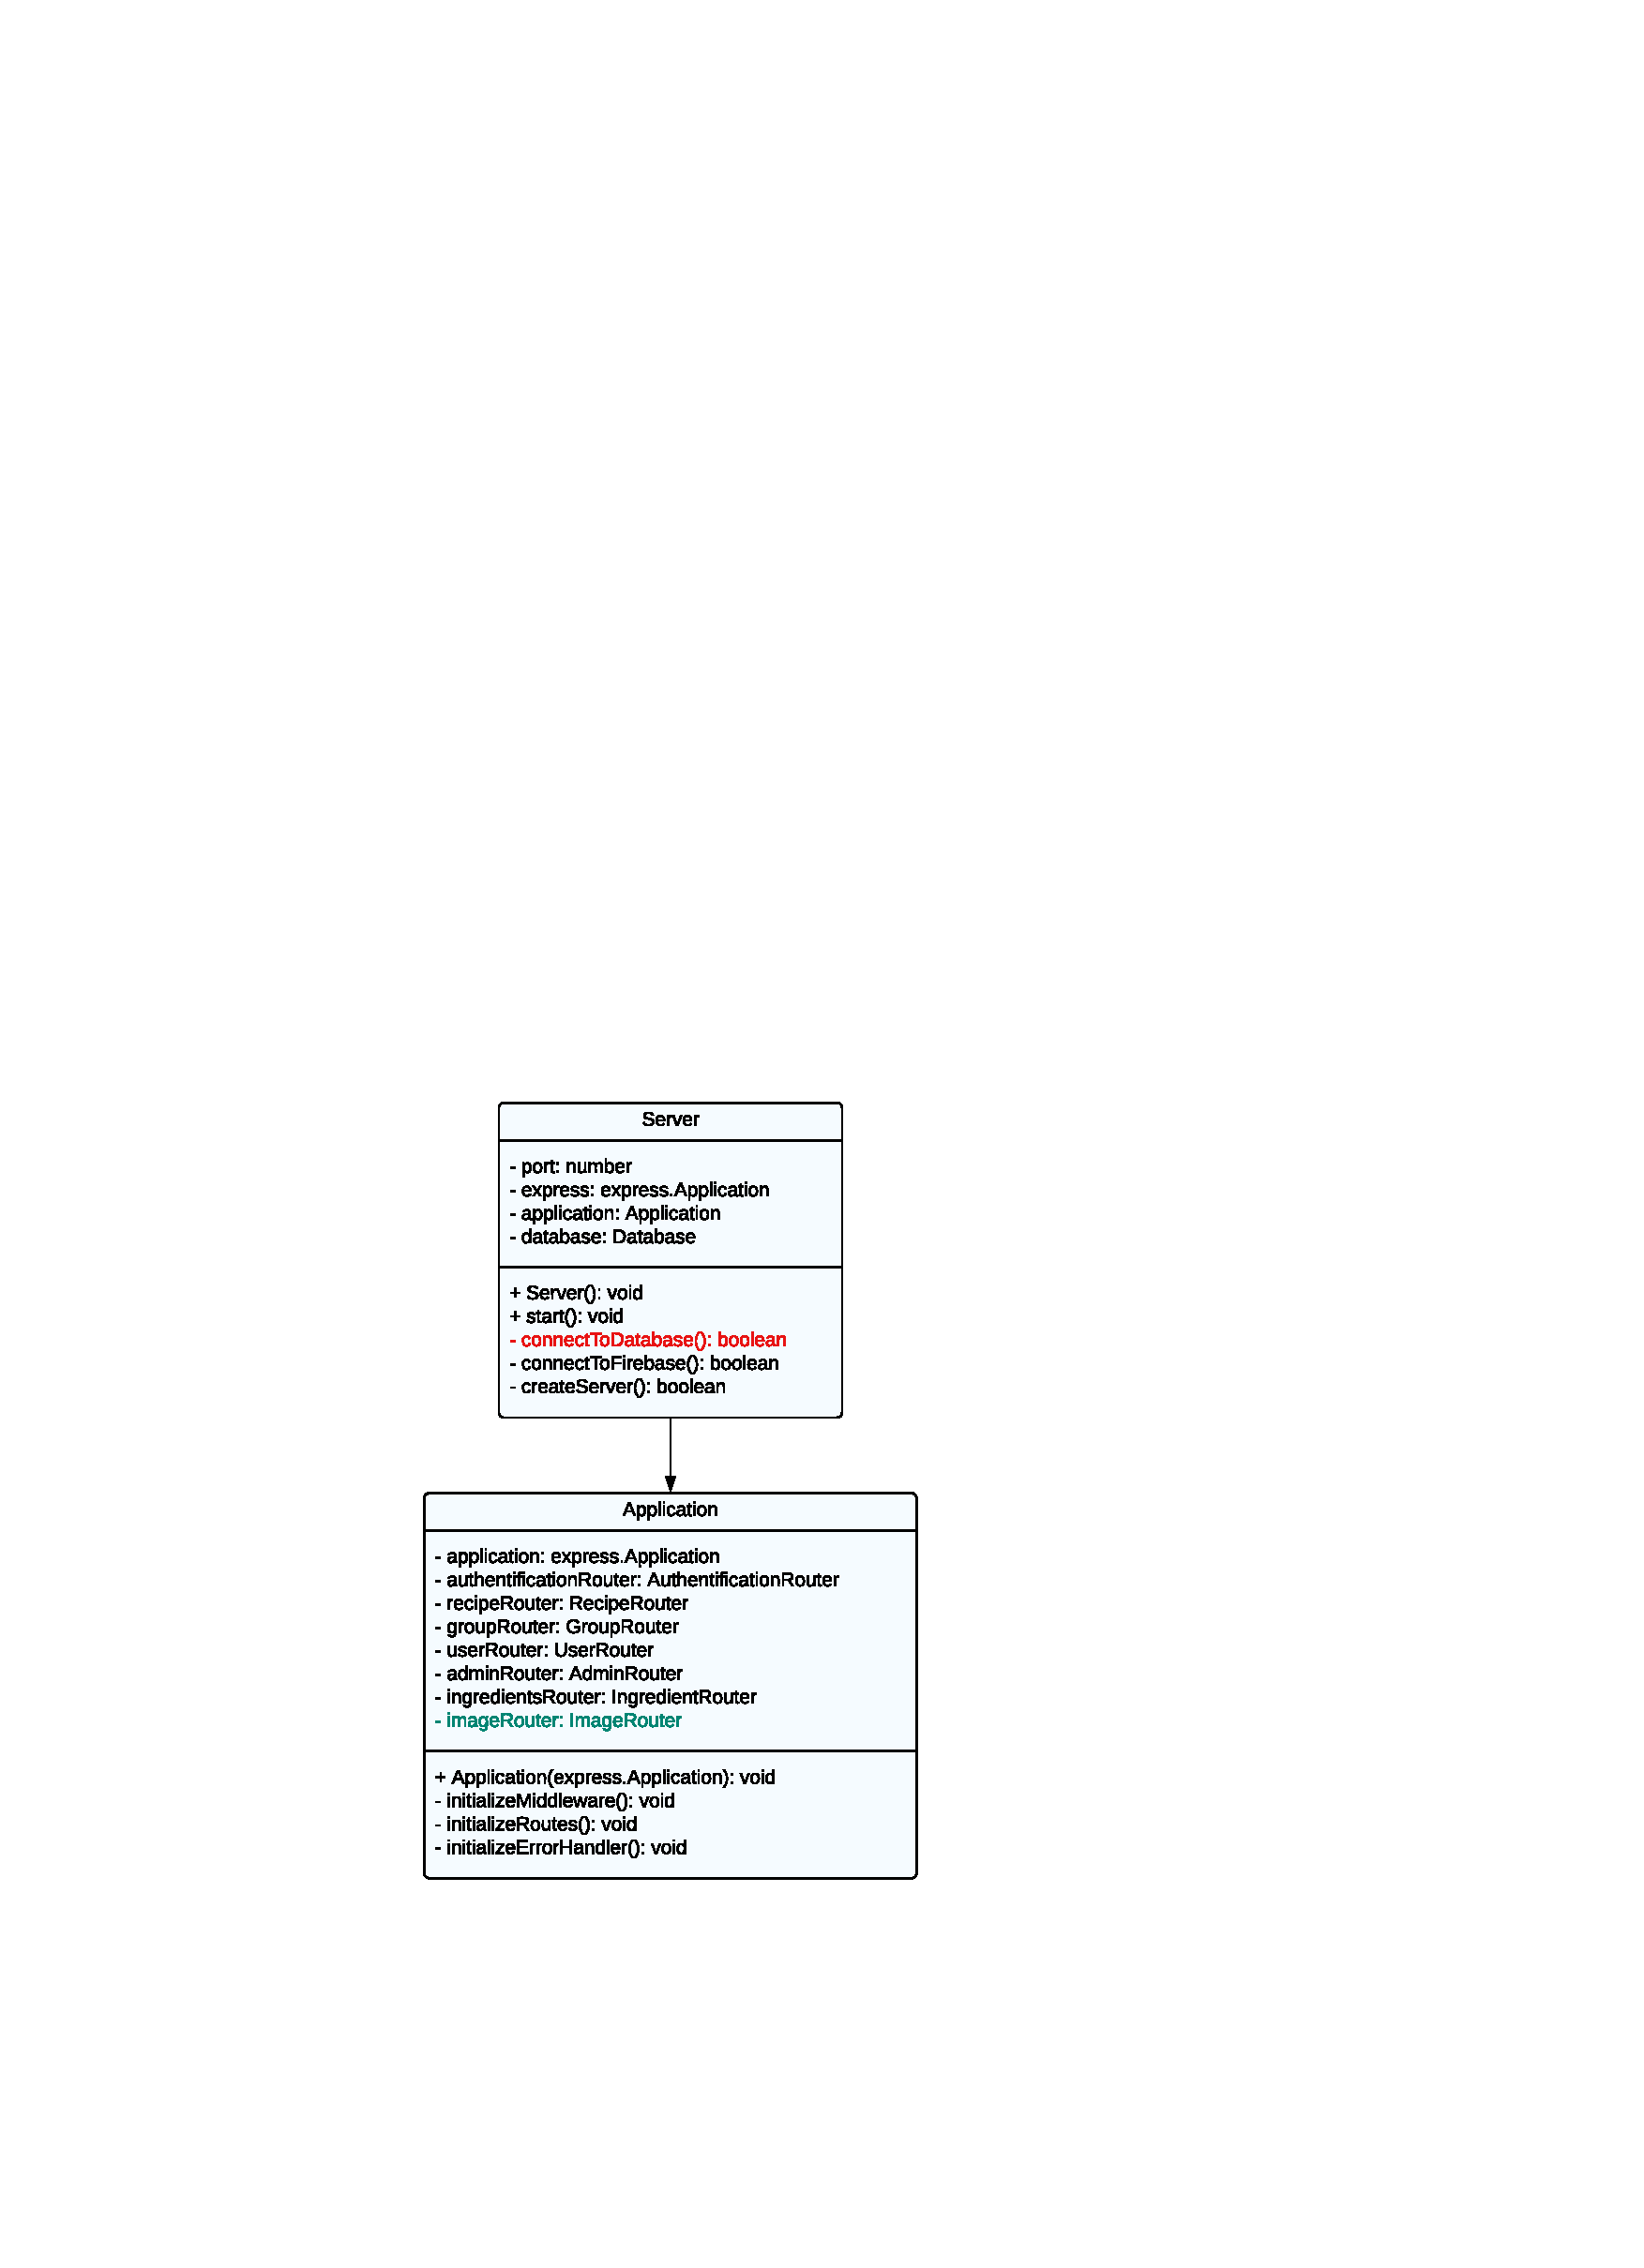
\includegraphics[width=0.95\textwidth]{images/uml/server.pdf}
    \caption{Änderungen an der Server- und Applicationklasse}
    \label{fig:server}
\end{figure}
\paragraph{\texttt{connectToDatabase()}} Die Methode wurde entfernt, da sie nicht mehr benötigt wird.

\paragraph{\texttt{imageRouter: ImageRouter}} Die Attribute wurde hinzugefügt um die ImageRouter-Klasse zu initialisieren.

\subsection{Änderungen an den Routern}
\begin{figure}[htp]
    \centering
    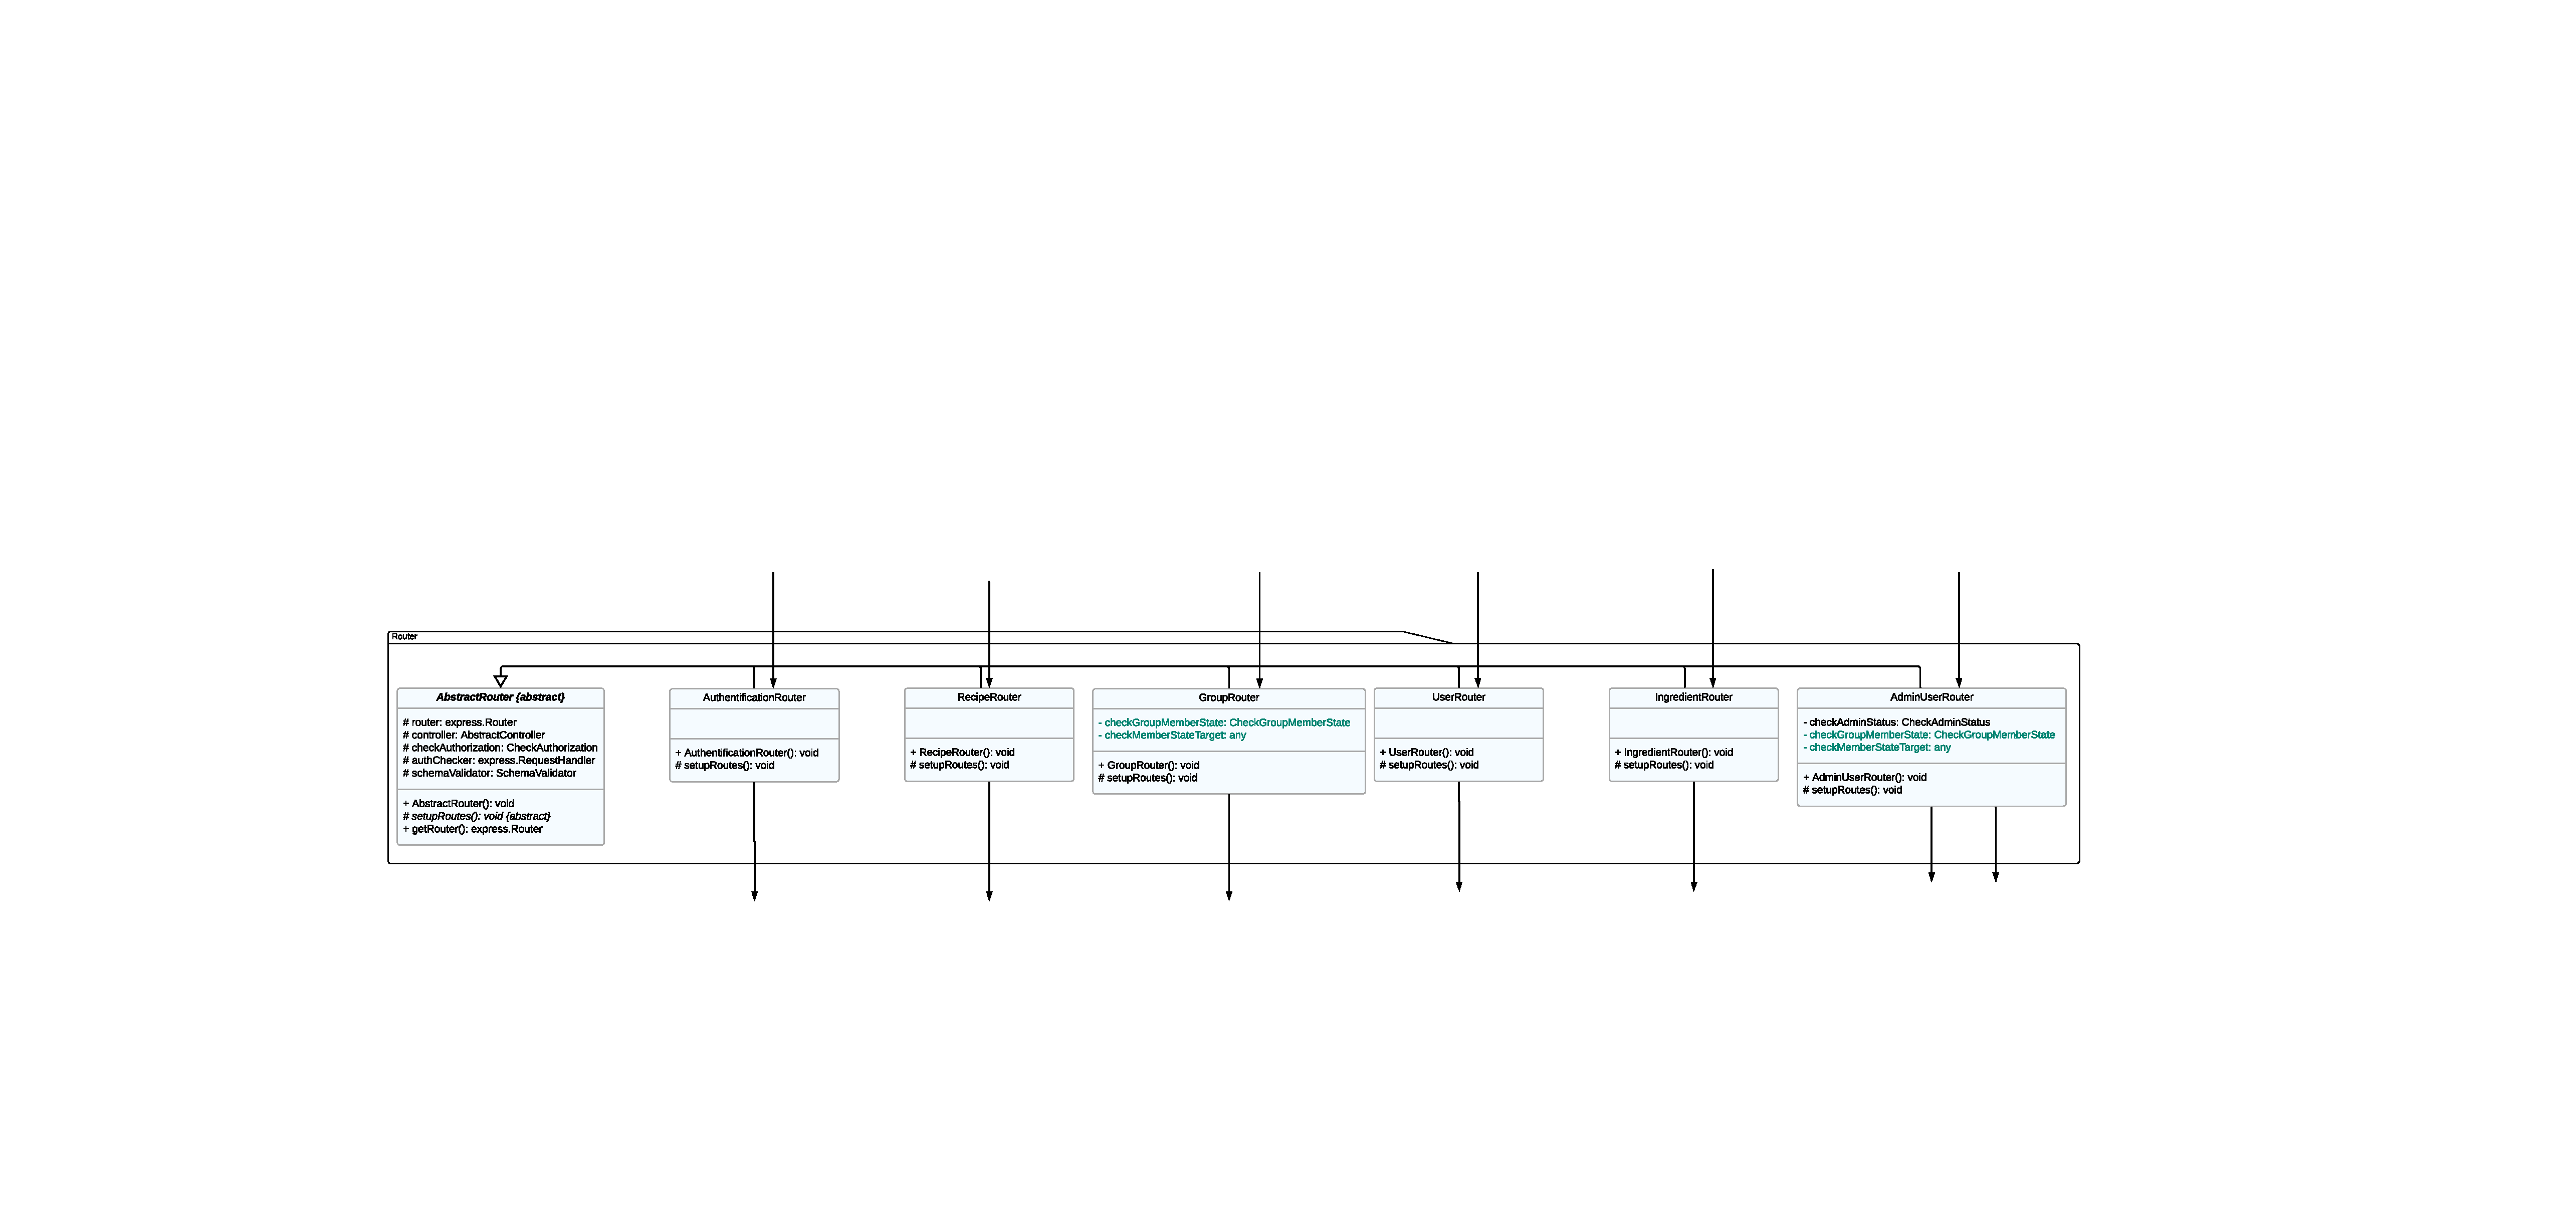
\includegraphics[width=0.95\textwidth]{images/uml/routers.pdf}
    \caption{Änderungen an den Routern}
    \label{fig:routers}
\end{figure}

Es wurden sowohl bei dem \texttt{GroupRouter} als auch beim \texttt{AdminUserRouter} folgende Attribute hinzugefügt.

\paragraph{\texttt{checkGroupMemberState: CheckGroupMemberState}} Die Attribute wurde hinzugefügt um die CheckGroupMemberState-Klasse zu initialisieren.
\paragraph{\texttt{checkMemberStateTarget: any}}

\newpage

\subsection{Änderungen an den Controllern}

\begin{figure}[htp]
    \centering
    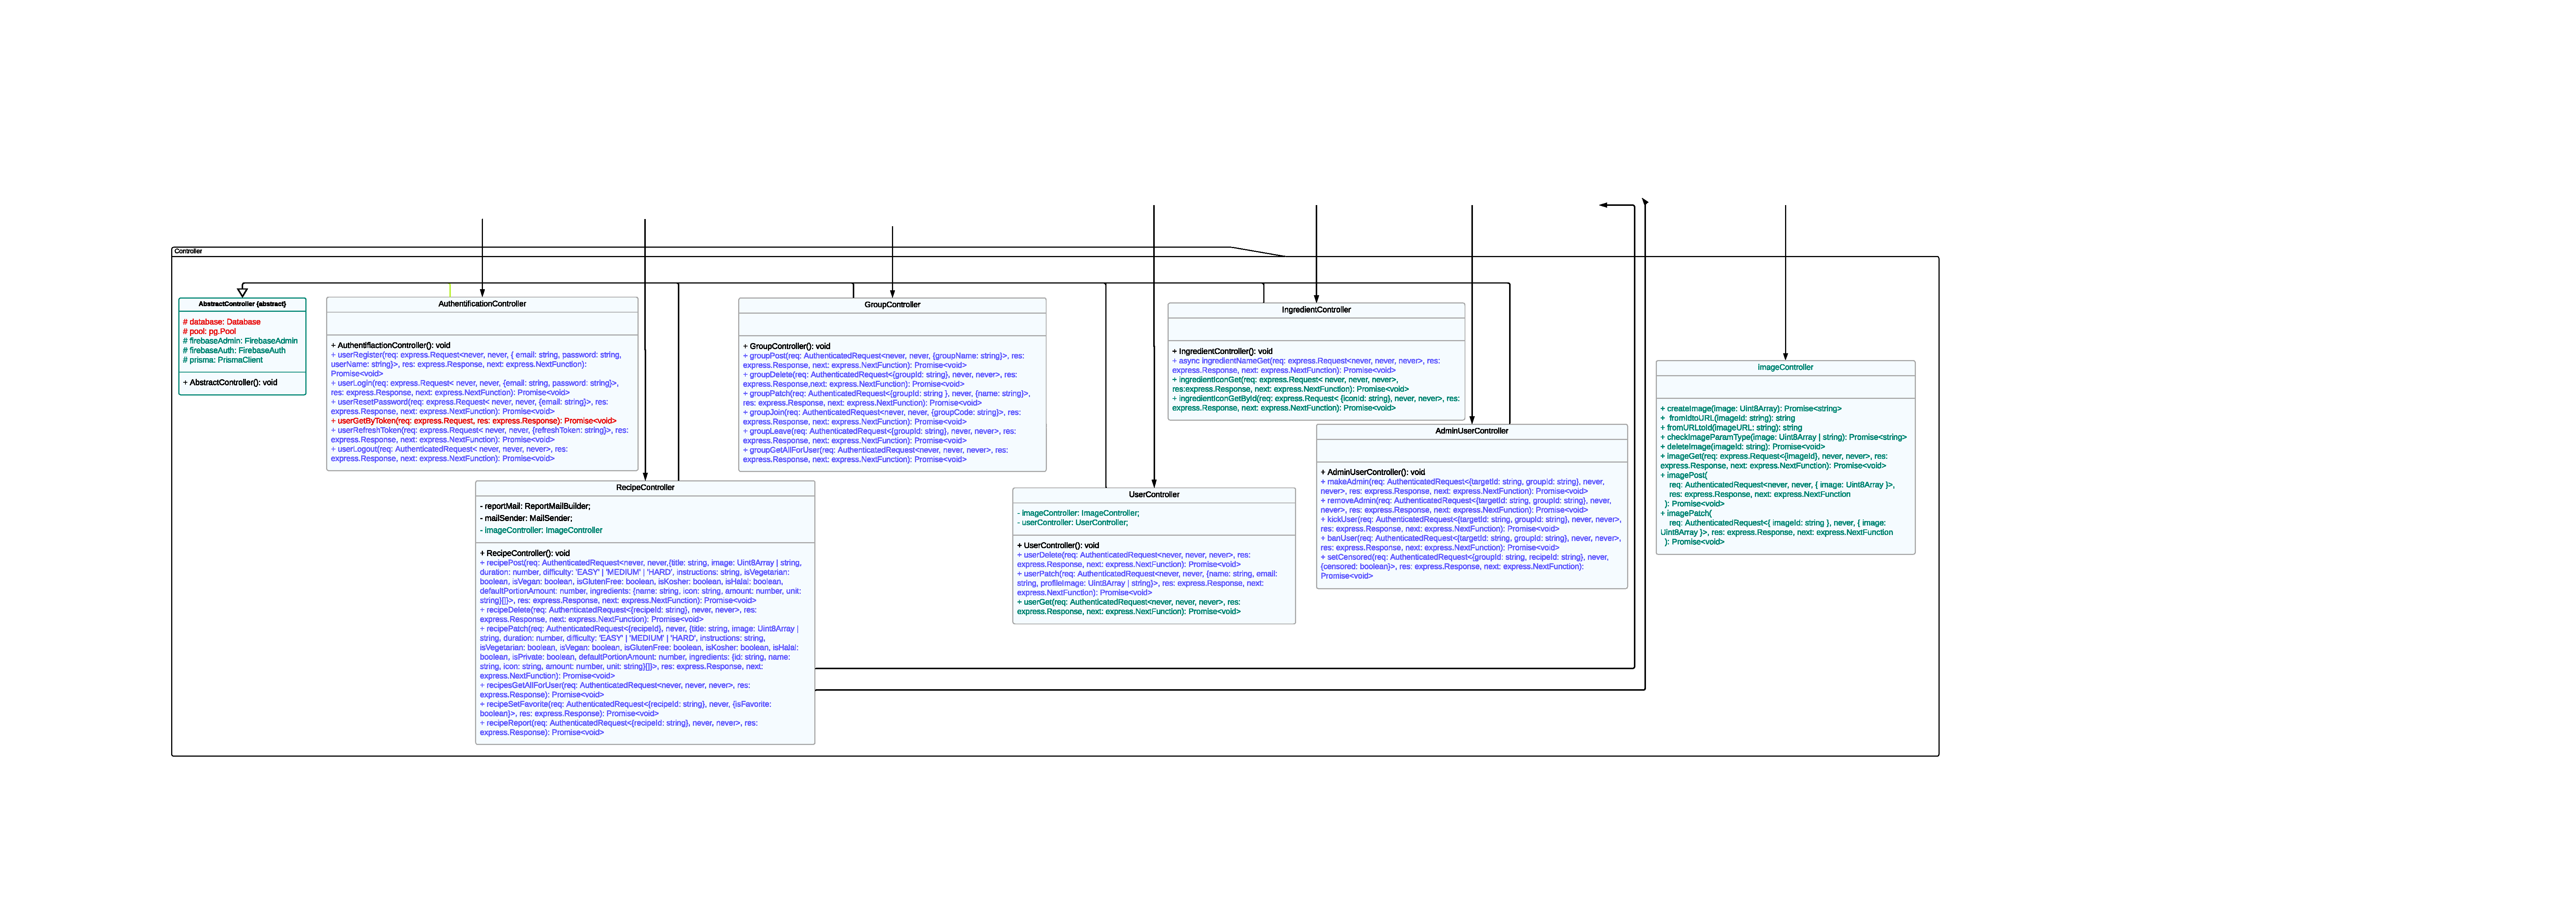
\includegraphics[width=0.95\textwidth]{images/uml/controller.pdf}
    \caption{Änderungen an den Controllern}
    \label{fig:controller}
\end{figure}

Bei allen Controllerfunktionen wurde das Request-Argument typsicher gemacht, d.h. es ist klar definiert, welche Argumente in head und body übergeben werden.
Außerdem werden eventuell auftretende Fehler mit der next function an den Errorhandler weitergegeben. Die Klasse \texttt{ImageController} wurde hinzugefügt, um Bilder zu verwalten.
\texttt{RecipeController} und \texttt{UserController} halten eine Instanz von \texttt{Imagecontroller}

\paragraph{\texttt{AbstractController}} Die Attribute \texttt{pool} und \texttt{database} wurden entfernt. Datenbankanfragen werden nun mithilfe des PrismaClients über das Attribut \texttt{prisma} ausgeführt.
Außerdem wurden die Attribute \texttt{firebaseAuth} und \texttt{firebaseAdmin} hinzugefügt, um die Authentifizierung mit Firebase zu ermöglichen.

\paragraph{\texttt{UserController}} Die Methode getUser wurde hinzugefügt, um einen Benutzer anhand seines idTokens zu erhalten.

\paragraph{\texttt{AuthentificationController}} Die Methode \texttt{userGetByIdToken} wurde entfernt und durch die Methode \texttt{getUser} im UserController ersetzt.

\paragraph{\texttt{IngredientController}} Die Methode \texttt{ingredientIconGet} wurde hinzugefügt, um alle Icons als URL zu erhalten. Die Methode \texttt{ingredientIconGetById} wurde hinzugefügt, um ein Icon anhand seiner ID als Bytearray zu erhalten.

\paragraph{\texttt{GroupController}} Dieser Controller hält nun Instanzen von Ingredient und Image Controller.

\paragraph{\texttt{ImageController}} Diese Klasse wurde hinzugefügt, um Bilder zu verwalten. Sie enthält die folgenden Methoden:
\begin{itemize}
    \item \texttt{createImage(image:UInt8Array)} um ein Bild zu erstellen.
    \item \texttt{imageGet(req: express.Request<{imageId:string},never,never>, res: express.Response, next: express.NextFunction)} um ein Bild anhand seiner ID zu erhalten.
    \item \texttt{fromIdtoURL(imageId: string): string} gibt für image id die URL zurück.
    \item \texttt{fromURLtoId(imageURL: string): string} gibt für image URL die ID zurück.
    \item \texttt{checkImageParamType(image: UInt8Array|string)} um ein Bild hochzuladen.
    \item \texttt{deleteImage(req: express.Request<{imageId:string},never,never>, res: express.Response, next: express.NextFunction)} um ein Bild anhand seiner ID zu löschen.
    \item \texttt{imagePost(req: AuthenticatedRequest<never, never, { image: Uint8Array }>,res: express.Response, next: express.NextFunction): Promise<void>} um ein Bild hochzuladen.
    \item \texttt{imagePatch(req: AuthenticatedRequest<{ imageId: string }, never, { image: Uint8Array }>, res: express.Response, next: express.NextFunction): Promise<void>} um ein Bild anhand seiner ID zu aktualisieren.
\end{itemize}

\subsection{Änderungen an der Middleware} Wie auch bei den Controllern, wurden auch bei der Middleware alle Request-Argumente typsicher gemacht. Die Klassen \texttt{AbstractMiddleware}, \texttt{CheckGroupMemberState}, \texttt{SchemaValidator} und \texttt{AuthenticatedRequest} wurden neu hinzugefügt.


\begin{figure}[htp]
    \centering
    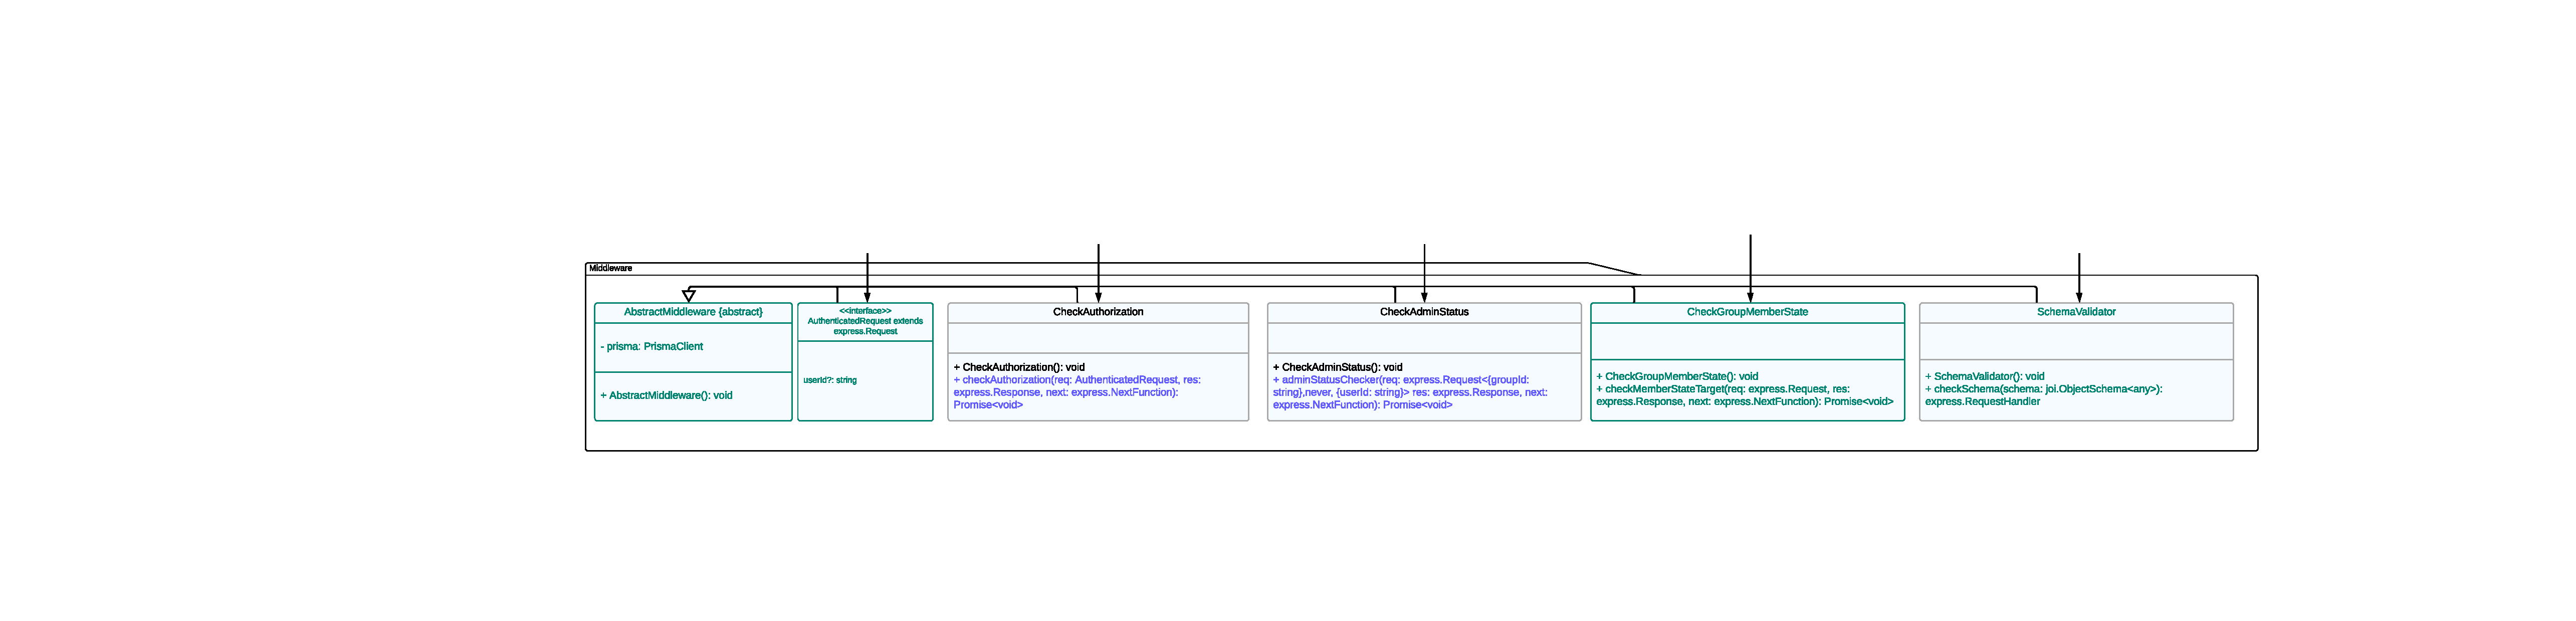
\includegraphics[width=0.95\textwidth]{images/uml/middleware.pdf}
    \caption{Änderungen an den Middlewareklassen}
    \label{fig:middleware}
\end{figure}

\paragraph{\texttt{AbstractMiddleware}} Klasse, von der alle anderen Middlewareklassen erben. Sie enthält einen Constructor und das Attribut \texttt{prisma : PrismaClient} um Datenbankanfragen auszuführen.

\paragraph{\texttt{AuthenticatedRequest}} Interface, das \texttt{express.Request} um das Atrribut \texttt{userId : string} erweitert.

\paragraph{\texttt{CheckGroupMemberState}} Klasse, die überprüft, ob ein Benutzer Mitglied einer Gruppe ist. Dazu wird die Methode \\ \texttt{checkMemberStateTarget(express.Request, express.Response, express.NextFunction)} verwendet.

\paragraph{\texttt{SchemaValidator}} Klasse, die die Requestdaten anhand eines Joi-Schemas validiert. Dazu wird die Methode \texttt{validateRequest(schema: joi.objectSchema)} verwendet.
Bei der Entwicklung von TypeScript-Anwendungen ist die Dateneingabevalidierung von entscheidender Bedeutung, um die Integrität und Sicherheit unserer Anwendung zu gewährleisten. Die Bibliothek Joi hat sich als eine der beliebtesten und effektivsten Lösungen für die Validierung von Daten in JavaScript erwiesen. Wir haben uns deshalb für diese leistungsstarke Validierungs-Bibliothek entschieden haben.
Alle Request, die gestellt werden können werden dabei mit Joi validiert. Dabei wird überprüft, ob alle benötigten Felder vorhanden sind und ob die Felder den richtigen Datentyp haben.

Dafür hat jeder Controller ein Joi-Schema, das die Validierung beschreibt. Dieses Schema wird dann in der \texttt{validateRequest}-Middleware verwendet, um die Request zu validieren.

\paragraph{\texttt{CheckAuthorization}} Die Methode \texttt{checkAuthorization} findet nun zusätzlich den Nutzer in der Datenbank und fügt seine Id der Request hinzu. Weitergegeben wird eine \texttt{AuthenticatedRequest}.

\newpage

\subsection{MailBuilder} Die Methode \texttt{buildMail(reciever: string, adminUsername: string, recipeTitle: string, reportedUsername: string, groupName: string): nodemailer.SendMailOptions} erstellt eine zu sendende Mail.


\begin{figure}[htp]
    \centering
    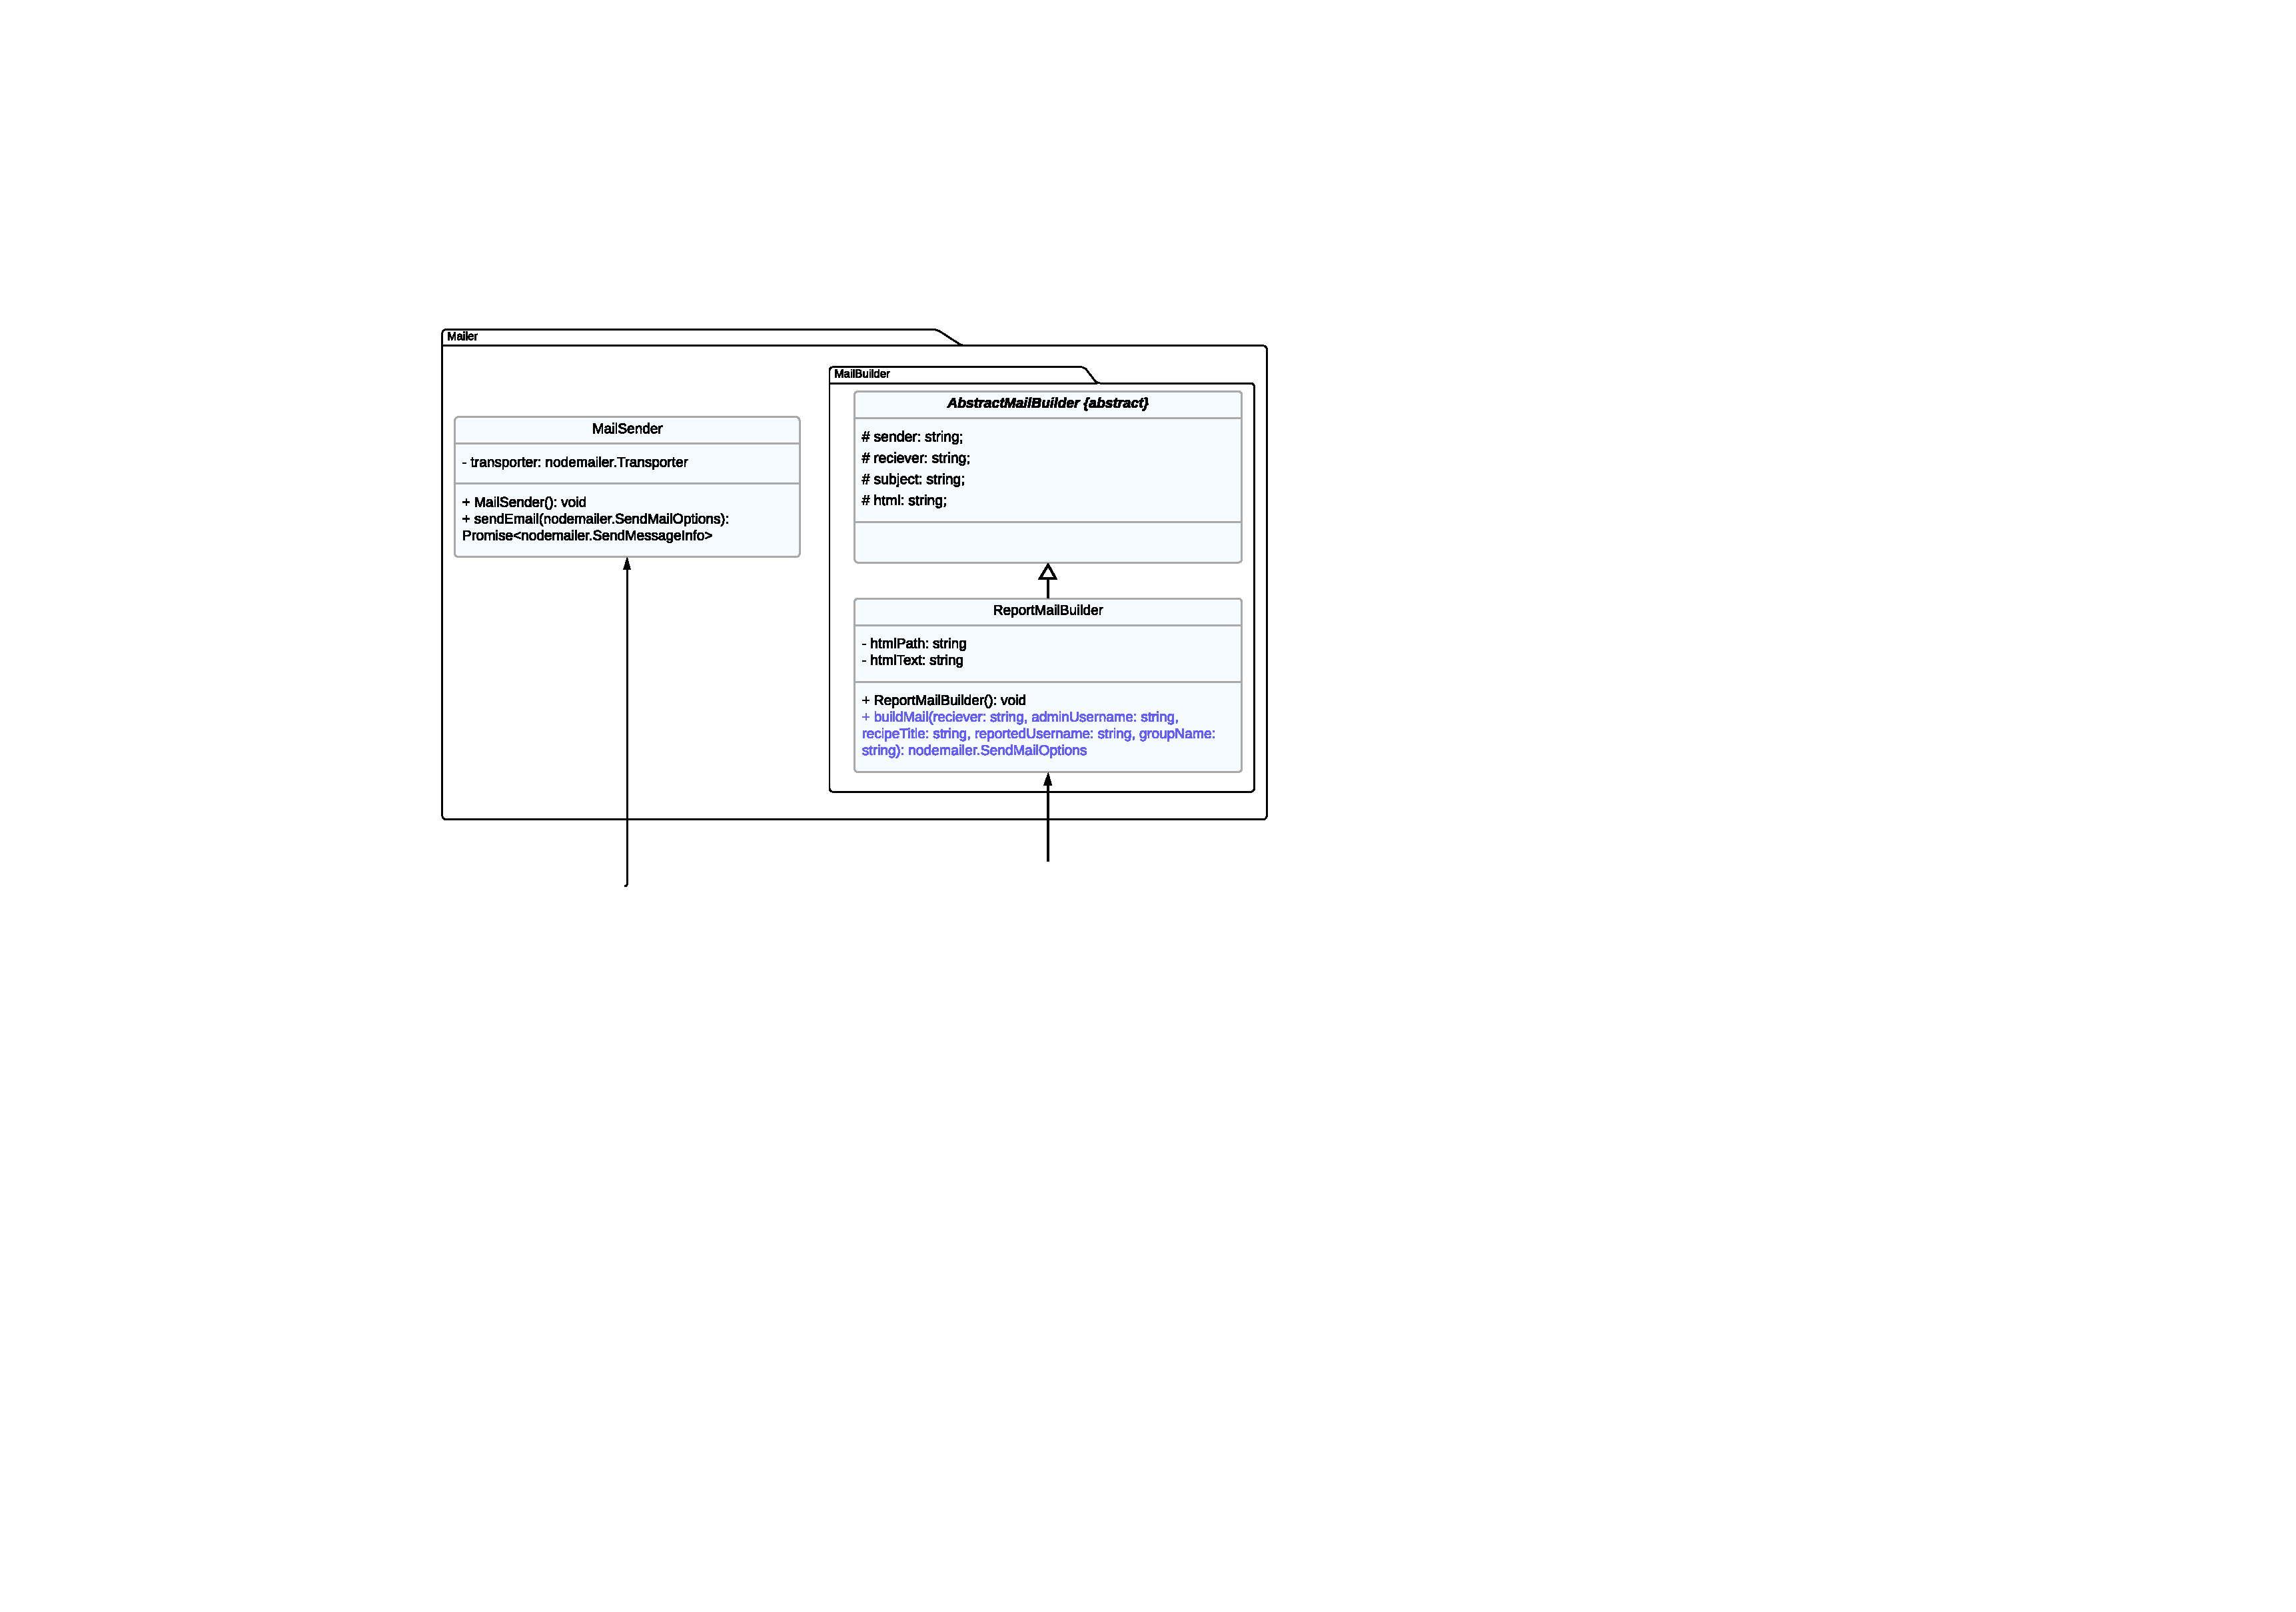
\includegraphics[width=0.95\textwidth]{images/uml/mailbilder.pdf}
    \caption{Änderungen am Mailbuilder}
    \label{fig:mailbuilder}
\end{figure}


\subsection{Database} Table User, Recipe und Ingredient halten nun nur noch die UUID ihres Bildes bzw Icons. Die Bilder und Icons werden in neuen Tables gespeichert.

\paragraph{Image} Neuer Table, in dem Images anhand uuid in Byteform gespeichert werden.

\paragraph{IngredientIcon}  Neuer Table, in dem Icons anhand uuid in Byteform gespeichert werden. Der Table enthält außerdem ein Feld für den Namen des Icons.

\begin{figure}[htp]
    \centering
    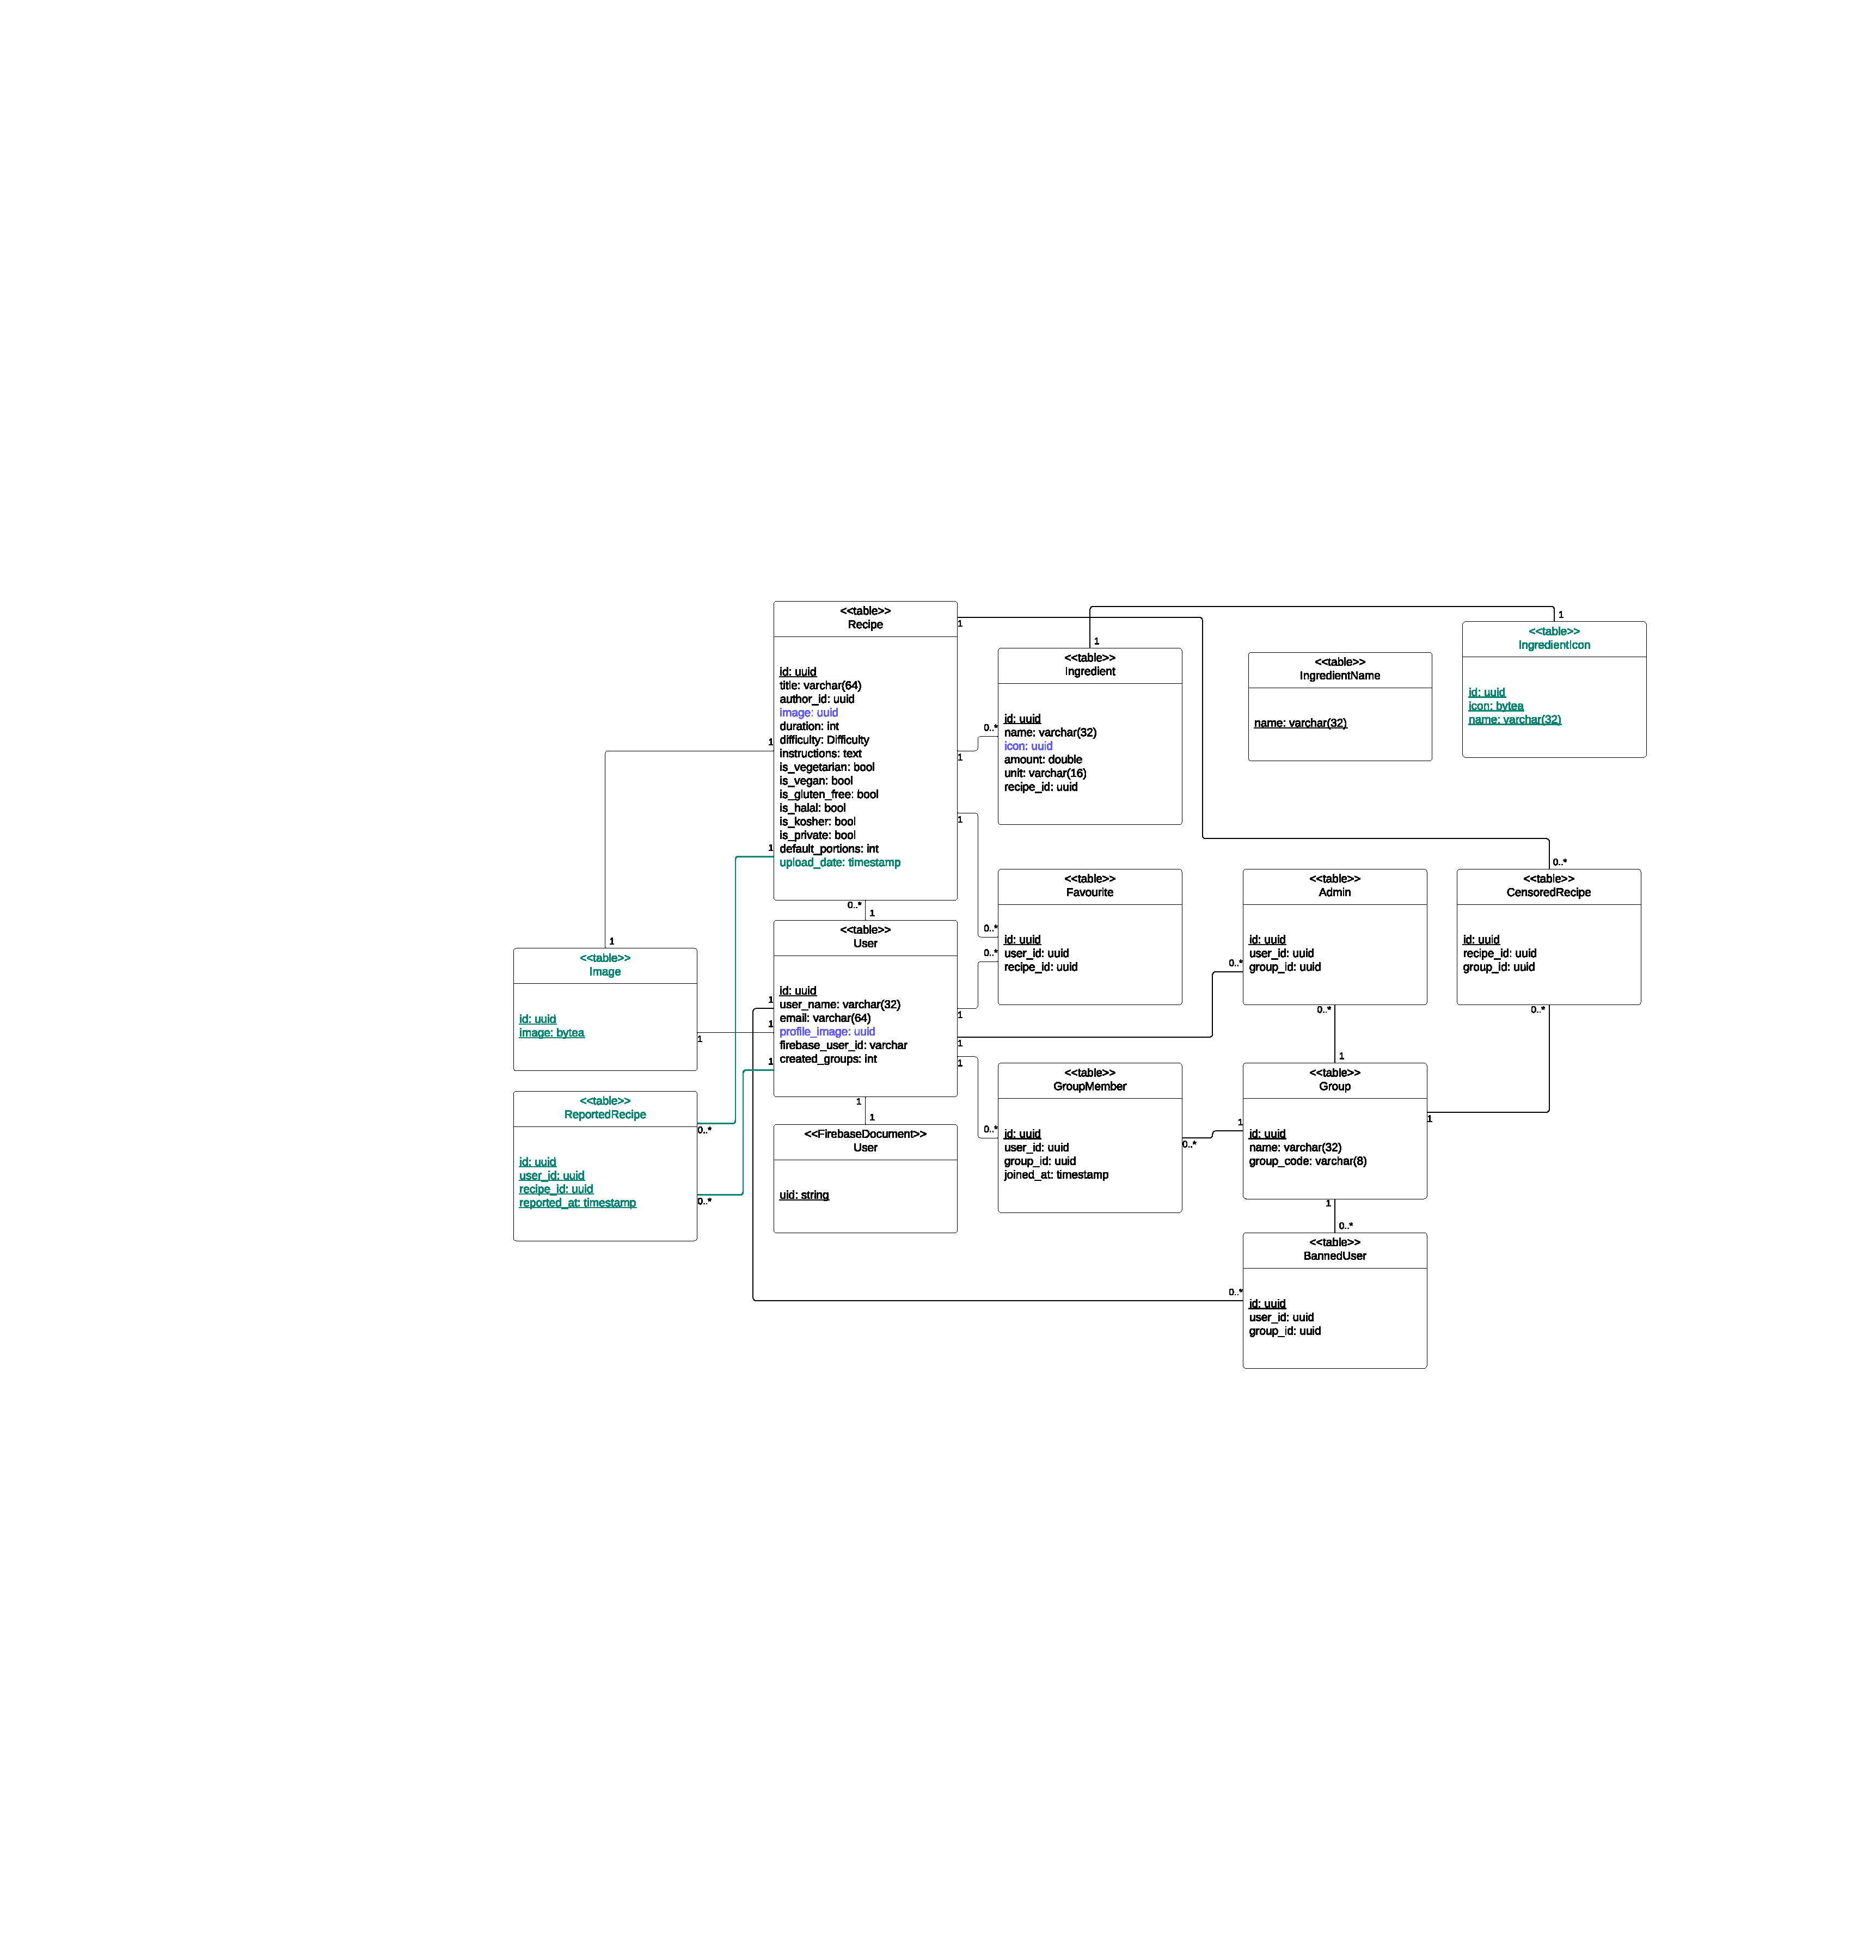
\includegraphics[width=0.95\textwidth]{images/uml/database.pdf}
    \caption{Änderungen an der Datenbank}
    \label{fig:database}
\end{figure}
\newpage

\section{Grafische Benutzeroberfläche}
Das Design der grafischen Benutzeroberfläche änderte sich nicht wesentlich von dem, was wir uns im Pflichtenheft überlegt hatten.
Es kam nur zu kleinen Änderungen, wie sie im Kapitel \ref{sec:changes} beschrieben sind.

\newpage

\end{document}